\documentclass[10pt]{beamer}
\setbeamertemplate{navigation symbols}{}
\usepackage{graphicx}
%\usepackage{feynmp}
\usepackage{subfigure}
\graphicspath{{figs/}}
\usepackage{epsfig,psfrag,amssymb,amsmath,amsthm,amsbsy,setspace, hyperref}
\usepackage{xspace}
%\usepackage[titletoc]{appendix}
\usepackage{afterpage}
\usepackage{multirow}
\usepackage{footnpag}
\usetheme{Berkeley}
\useoutertheme{pete}
\usepackage{fancyhdr,color,mathrsfs}
\beamersetuncovermixins{\opaqueness<1>{25}}{\opaqueness<2->{15}}
\begin{document}
%\begin{fmffile}{petes_defense_mp}
\renewcommand{\thefootnote}{\fnsymbol{footnote}}

\newcommand{\ud}{\mathrm{d}}
\newcommand{\m}{\mathrm{m}}
\newcommand{\lqcd}{\ensuremath{\Lambda_{QCD} }}
\newcommand{\red}[1]{ \textcolor{red}{#1} }
\newcommand{\blue}[1]{\textcolor{blue}{#1}}
%\newcommand{\red}[1]{}
%\newcommand{\blue}[1]{}
\setlength{\unitlength}{1cm}
\newcommand{\cmt}[1]{}
 \def\intL{\ensuremath{{\cal L}}} %\mathcal{L}}
 
 \newcommand{\su}[1]{\ensuremath{SU(#1)}}
 \newcommand{\so}[1]{\ensuremath{SO(#1)}}
 \newcommand{\uu}[1]{\ensuremath{U(#1)}}
% \newcommand{\su2}{\ensuremath{SU(2)}}
\newcommand{\qcd}{QCD}  
\newcommand{\alphas}{\ensuremath{\alpha_s}} 
%\newcommand{\alpgen}{ALPGEN\xspace}
%\newcommand{\jimmy}{JIMMY\xspace}
\newcommand{\NLOJET}{NLOJET++\xspace}
\newcommand\powheg{{\tt P\scalebox{0.9}{OWHEG}}\xspace}
\newcommand\pythia{{\tt P\scalebox{0.9}{YTHIA}}\xspace}
\newcommand\herwig{{\tt H\scalebox{0.9}{ERWIG}}\xspace}
\newcommand\alpgen{{\tt A\scalebox{0.9}{LPGEN}}\xspace}

\newcommand\POWHEG{{\tt P\scalebox{0.9}{OWHEG}}\xspace}
\newcommand\PYTHIA{{\tt P\scalebox{0.9}{YTHIA}}\xspace}
\newcommand\HERWIG{{\tt H\scalebox{0.9}{ERWIG}}\xspace}
\newcommand\jimmy{{\tt J\scalebox{0.9}{IMMY}}\xspace}
\newcommand\athena{{\tt A\scalebox{0.9}{thena}}\xspace}
\newcommand\atlas{{\tt A\scalebox{0.9}{TLAS}}\xspace}
\newcommand\cms{{\tt C\scalebox{0.9}{MS}}\xspace}
\newcommand\geant{{\tt G\scalebox{0.9}{EANT4}}\xspace}

\newcommand{\mass}{$m_{12}$}
 % cribbed from atlasphysics.sty
\def\pt{\ensuremath{p_{\mathrm{T}}}} % Subscript roman not italic (EE)
\def\pT{\ensuremath{p_{\mathrm{T}}}} % Subscript roman not italic (EE)
\def\et{\ensuremath{E_{\mathrm{T}}}} % Subscript roman not italic (EE)
\def\eT{\ensuremath{E_{\mathrm{T}}}} % Subscript roman not italic (EE)
\def\ET{\ensuremath{E_{\mathrm{T}}}} % Subscript roman not italic (EE)
\def\HT{\ensuremath{H_{\mathrm{T}}}} % Subscript roman not italic (EE)
\def\ptsq{\ensuremath{p^2_{\mathrm{T}}}} % Fixed so it works correctly (EE)
%\def\akt{anti-kt}
\def\akt{\hbox{anti-${k_t}$}\xspace}
\def\kt{$k_t$\xspace}
 
 \def\moliere{Moli\`ere }


\title{Measurement of the inclusive jet and dijet cross sections using 2010 data from the ATLAS detector and calibration studies and simulation of the ATLAS forward calorimeter}%Pete's thesis defense}  
\author{Peter Thompson}
\date{\today} 
\begin{frame}
\titlepage
\end{frame}


%Hokay stuff below will need to be pruned. 20 minutes only



%%%%%%%%%%%%%%%%%%%%%%%%%%%%%%%%%%%%%%%%%%%%%%%%%%%%%%%%%%%%%%%%%%%

\begin{frame}\frametitle{Table of contents}\tableofcontents
\end{frame} 
%%%%%%%%%%%%%%%%%%%%%%%%%%%%%%%%%%%%%%%%%%%%%%%%%%%%%%%%%%%%%%%%%%
\section{The LHC}
\begin{frame}\frametitle{The Large Hadron Collider (LHC)} 
\includegraphics[width=0.7\linewidth,angle=0]{LHC.eps}
\begin{itemize}
\item 27 km circumference, 45-170 m underground
\item Design luminosity of $10^{34} \mathrm{cm}^2\mathrm{s}^{-1}$, COM energy 14 TeV
\item Achieved $2 \times 10^{31} \mathrm{cm}^2\mathrm{s}^{-1}$, 7 TeV COM during 2010.
\item \atlas, CMS multipurpose experiments
%\item ALICE (heavy ions), LHCb (B physics).
\end{itemize}


\end{frame}
%%%%%%%%%%%%%%%%%%%%%%%%%%%%%%%%%%%%%%%%%%%%%%%%%%%%%%%%%%%%%%%%%%%
%%%%%%%%%%%%%%%%%%%%%%%%%%%%%%%%%%%%%%%%%%%%%%%%%%%%%%%%%%%%%%%%%%%

\section{The ATLAS Detector}
\begin{frame}\frametitle{The Atlas Detector} 
\begin{columns}
\column{0.75\linewidth}
\includegraphics[width=1.0\linewidth,angle=0]{Detector/ATLAS_overview}
\column{0.25\linewidth}
\begin{equation*}
\eta = - \log \tan \left(\frac{\theta}{2}\right)
\end{equation*}
\end{columns}
%\begin{columns}
%\column{0.7\linewidth}
\begin{itemize}
\item General purpose detector at the LHC
\item Inner Detector: charged particle tracking for $|\eta| < 2.5$
\item Calorimetry: energy measurement for $|\eta| < 4.9$
\item Muon Spectrometry: $|\eta| < 2.7$
\end{itemize}
%\column{0.3\linewidth}
%\begin{equation*}
%\eta = - \log \tan \left(\frac{\theta}{2}\right)
%\end{equation*}
%\end{columns}
\end{frame}
%%%%%%%%%%%%%%%%%%%%%%%%%%%%%%%%%%%%%%%%%%%%%%%%%%%%%%%%%%%%%%%%%%%%
\begin{frame}
\subsection{Trigger}
\frametitle{Trigger} 
Trigger selects ``interesting'' events. Collisions occur at a rate of 40~MHz, events recorded at $\sim$400~Hz (bandwidth).
\begin{itemize}
\item Level 1 (L1) (hardware)
\begin{itemize}
\item Calorimeter Trigger (L1Calo)
\begin{itemize}
\item Jet triggers (will be discussed later)
%\item Transverse Energy
\end{itemize}
\item Muon Trigger (L1Muon)
\item Decision required within 2.5~$\mu$s
\end{itemize}
\item High Level Trigger (HLT) (software)
\begin{itemize}
\item Level 2 (L2)
\begin{itemize}
\item Decision required in 40~ms
\end{itemize}
\item Event Filter (EF) 
\begin{itemize}
\item Decision required in 4~s
\item Not used in 2010
\end{itemize}
\end{itemize}
\end{itemize}

\end{frame}
%%%%%%%%%%%%%%%%%%%%%%%%%%%%%%%%%%%%%%%%%%%%%%%%%%%%%%%%%%%%%%%%%%%
%%%%%%%%%%%%%%%%%%%%%%%%%%%%%%%%%%%%%%%%%%%%%%%%%%%%%%%%%%%%%%%%%%%
\subsection{Forward Calorimeter}
\begin{frame}\frametitle{The Atlas Forward Calorimeters} 
\begin{columns}
\column{0.5\linewidth}
\begin{itemize}
\item Consist of one EM module (FCal1) and 2 hadronic modules (FCal2 and FCal3).
\item Covers pseudorapidity range $3.1 < |\eta| < 4.9$, approx 5m from IP.
%\item Liquid argon based calorimetery.
\item High particle flux at large $|\eta|$ requires novel design.
\begin{itemize}
\item Liquid Argon (LAr) gaps are much smaller than for conventional calorimeters.
\end{itemize}
\item Located in a region not covered by tracking, in-situ studies are difficult.
\end{itemize}
\column{0.5\linewidth}
\includegraphics[width=0.8\linewidth,angle=0]{Detector/ATLAS_overview_fcal.eps}\\
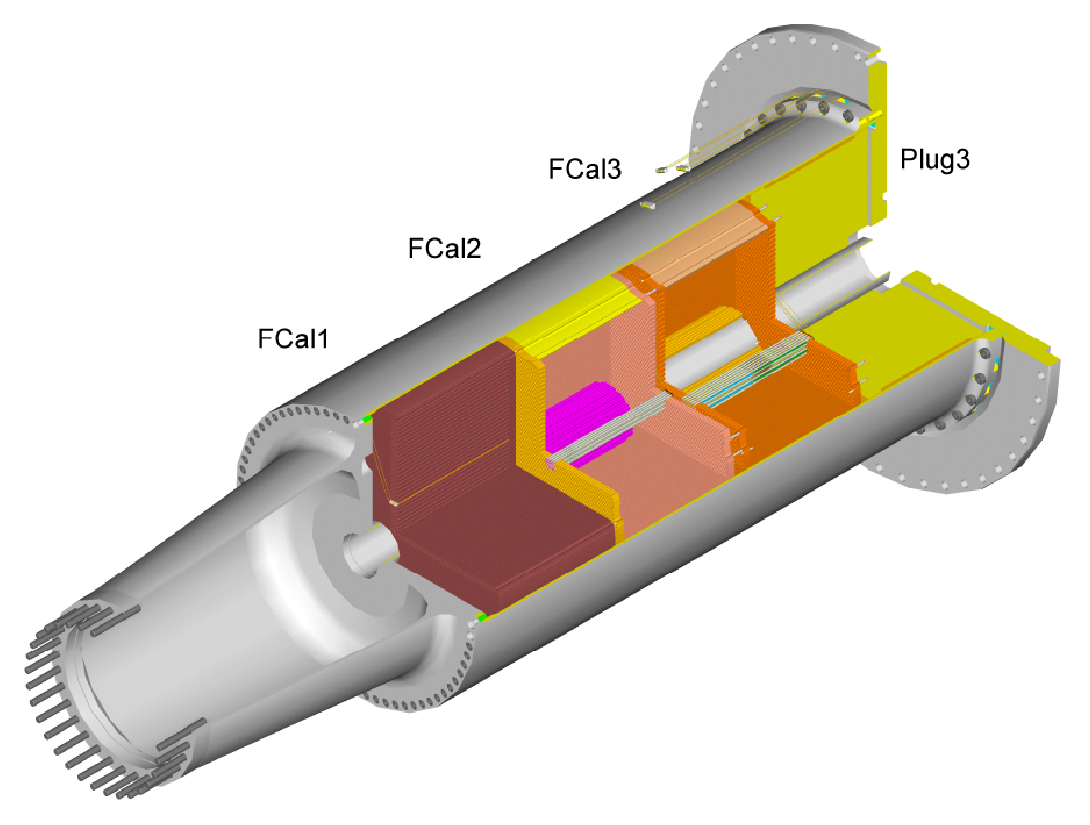
\includegraphics[width=0.8\linewidth,angle=0]{/TBoverview/FCal_support_cutaway.eps}
\end{columns}
\end{frame}
%%%%%%%%%%%%%%%%%%%%%%%%%%%%%%%%%%%%%%%%%%%%%%%%%%%%%%%%%%%%%%%%%%%%
\begin{frame}\frametitle{Hadronic Calibration} 
\begin{itemize}
\item First step in calibrating calorimeter is obtaining the ``EM scale'' calibration
\begin{itemize}
\item Calibrated response to photons, electrons.
\item Obtained from test beam studies.
\end{itemize}
\item Hadronic showers are more complex
\begin{itemize}
\item Part of the energy in a hadronic shower is ``invisible''.
\item EM component of the shower scales nonlinearly with the energy of initial hadron.
\item Calorimeter response non-linear with respect to energy of initial hadron.
\end{itemize}
\item Additional calibration required to reconstruct energy of hadronic particles.
\begin{itemize}
\item Simple method used for FCal beam test. 
\item More complex methods used at \atlas, derived from simulation.
\begin{itemize}
\item Requires a good simulation of the detector response.
\end{itemize}
\end{itemize}
\end{itemize}
%\item Liquid argon based calorimetery.
%\item High particle flux at large $|\eta|$ requires novel design.

\end{frame}
%%%%%%%%%%%%%%%%%%%%%%%%%%%%%%%%%%%%%%%%%%%%%%%%%%%%%%%%%%%%%%%%%%%%
%%\subsection{ FCal electrodes  }
%\begin{frame} 
%\frametitle{FCal electrodes} 
%\begin{columns}
%\column{0.6\linewidth}
%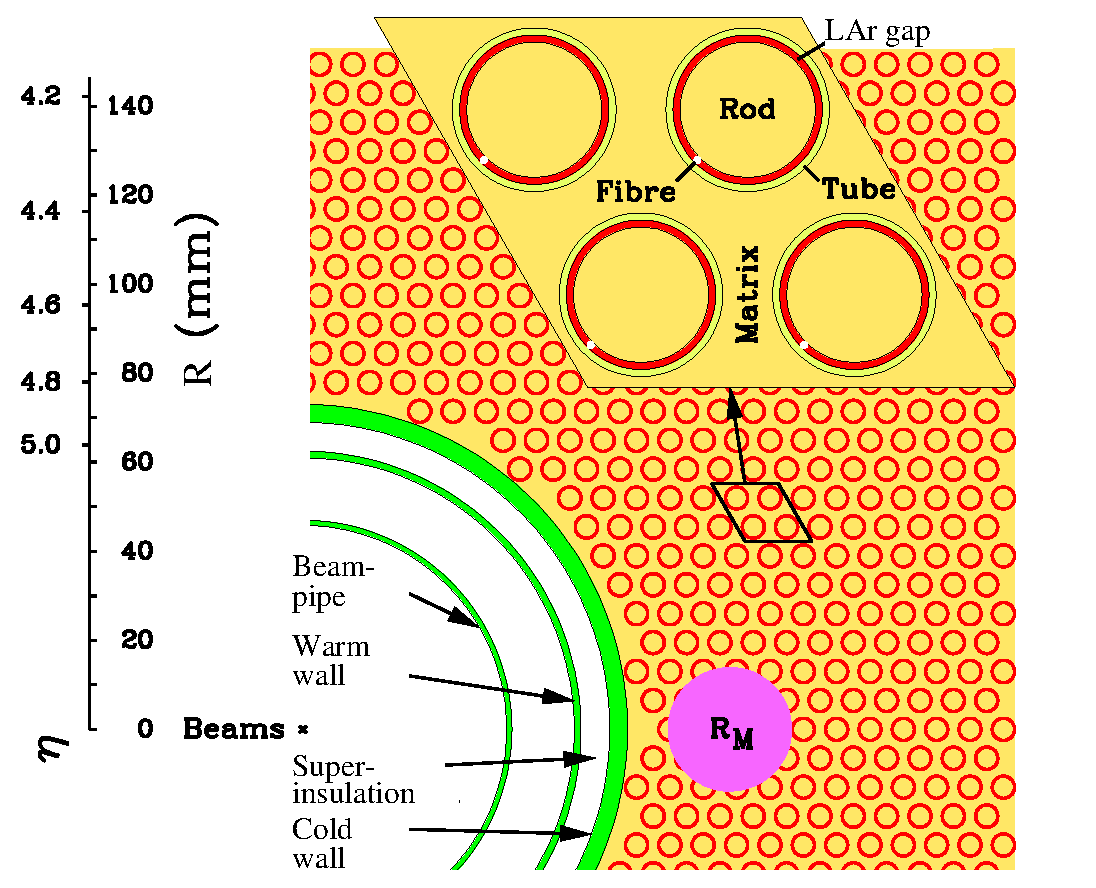
\includegraphics[width=0.8\linewidth,angle=0]{fcalfrontclose2.eps}\\
%\begin{itemize}
%\item Electrodes run down length of modules.
%\item Thin gaps between rod and tube occupied by LAr, sensitive regions.
%\item Absorbing material is copper in FCal1, tungsten based in FCal2 \& FCal3
%\end{itemize}
%\column{0.4\linewidth}
%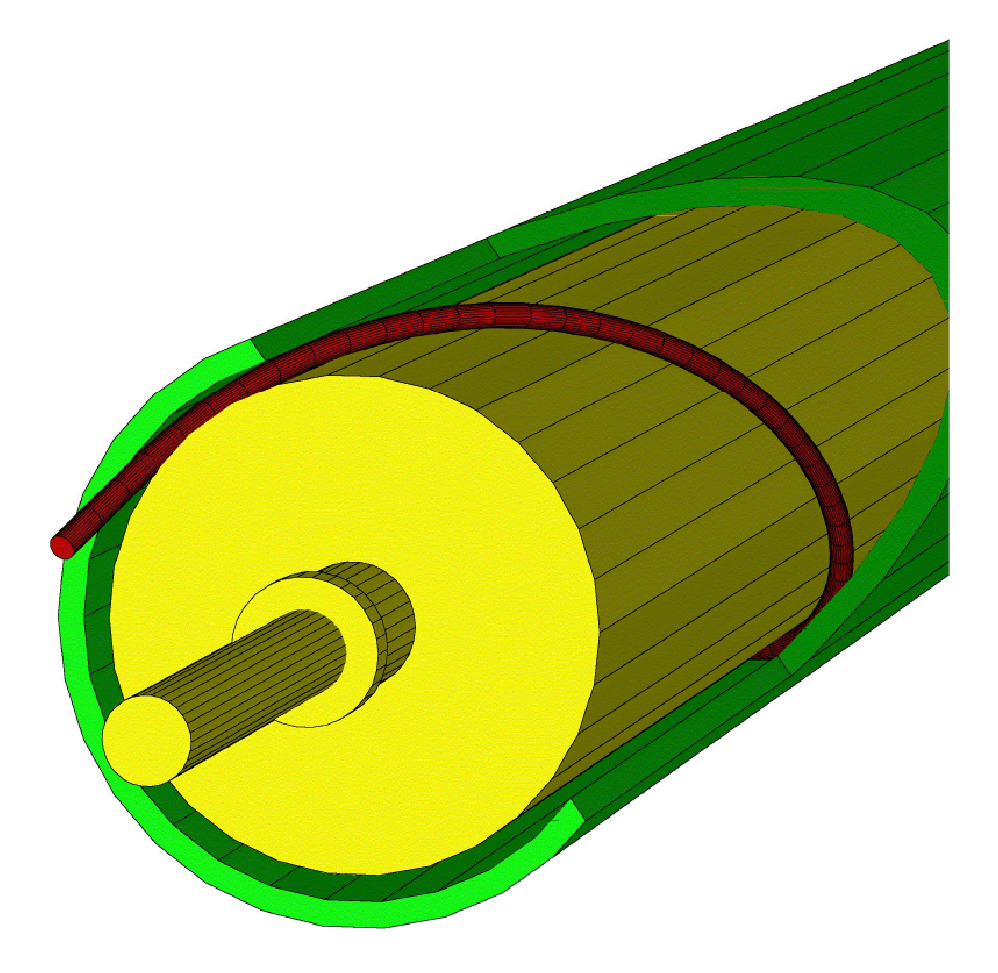
\includegraphics[width=0.8\linewidth,angle=0]{FCal_electrode.eps}\\
%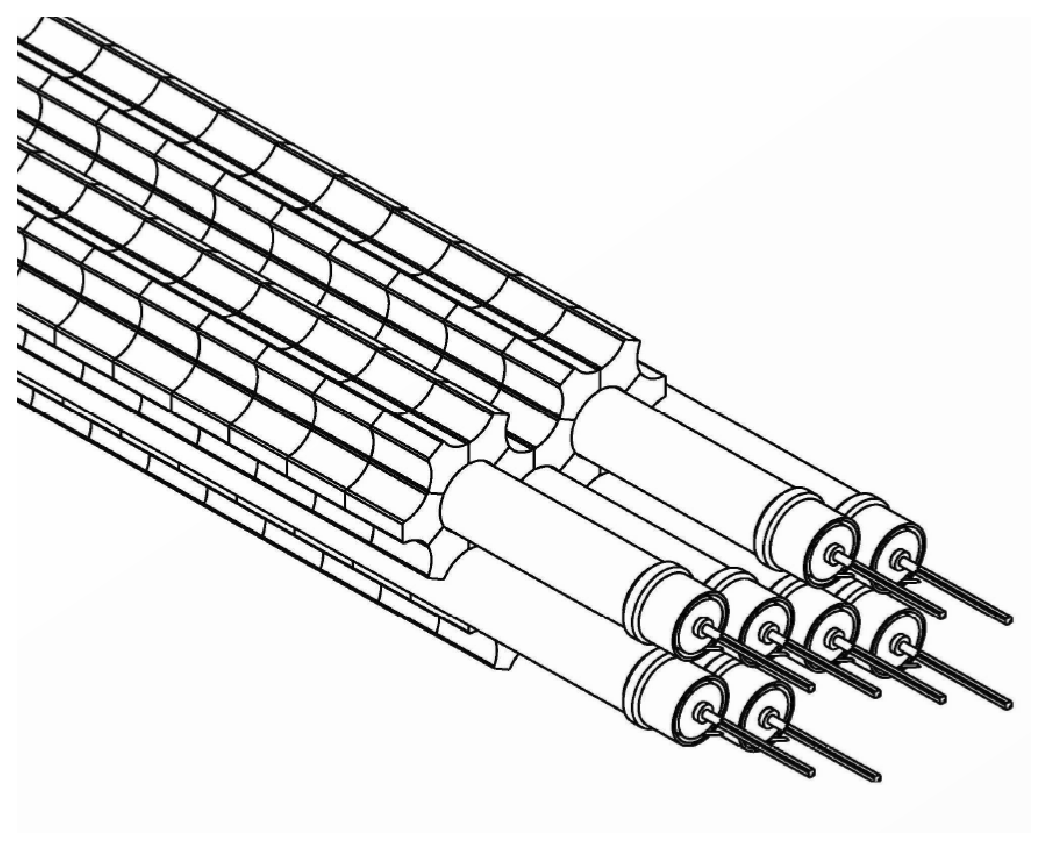
\includegraphics[width=0.8\linewidth,angle=0]{/TBoverview/rods_slugs.eps}
%\end{columns}
%\end{frame}
%%%%%%%%%%%%%%%%%%%%%%%%%%%%%%%%%%%%%%%%%%%%%%%%%%%%%%%%%%%%%%%%%%%%
\section{2003 Foward Calorimeter Beam Test}
\subsection{Test Beam Setup}
\begin{frame}\frametitle{Beam Test Motivation}
\begin{columns}
\column{0.55\linewidth}
\begin{itemize}
\item Obtain EM scale calibration (4L).
\item Study effect of additional material on detector performance:
\begin{itemize}
\item Response
\item Resolution
\end{itemize}
\item Validate Monte Carlo simulations of the FCal (4L/4H). 
\begin{itemize}
\item Performance
\item Shower shapes
\end{itemize}
\item FCal subjected to beams of electrons and hadrons at energies of 10-200 GeV.
\end{itemize}
\column{0.45\linewidth}
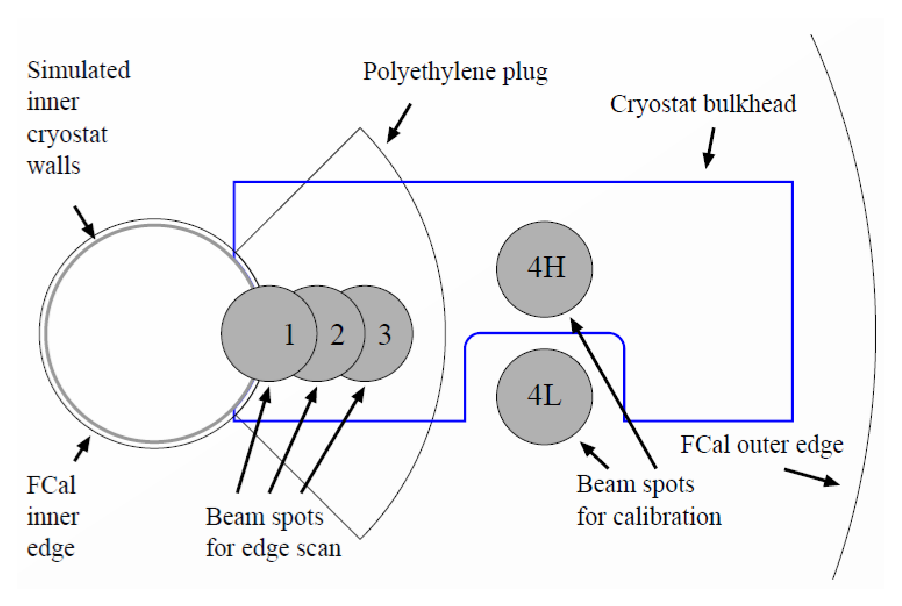
\includegraphics[width=1.0\linewidth,angle=0]{TB_beamspots.eps}\\
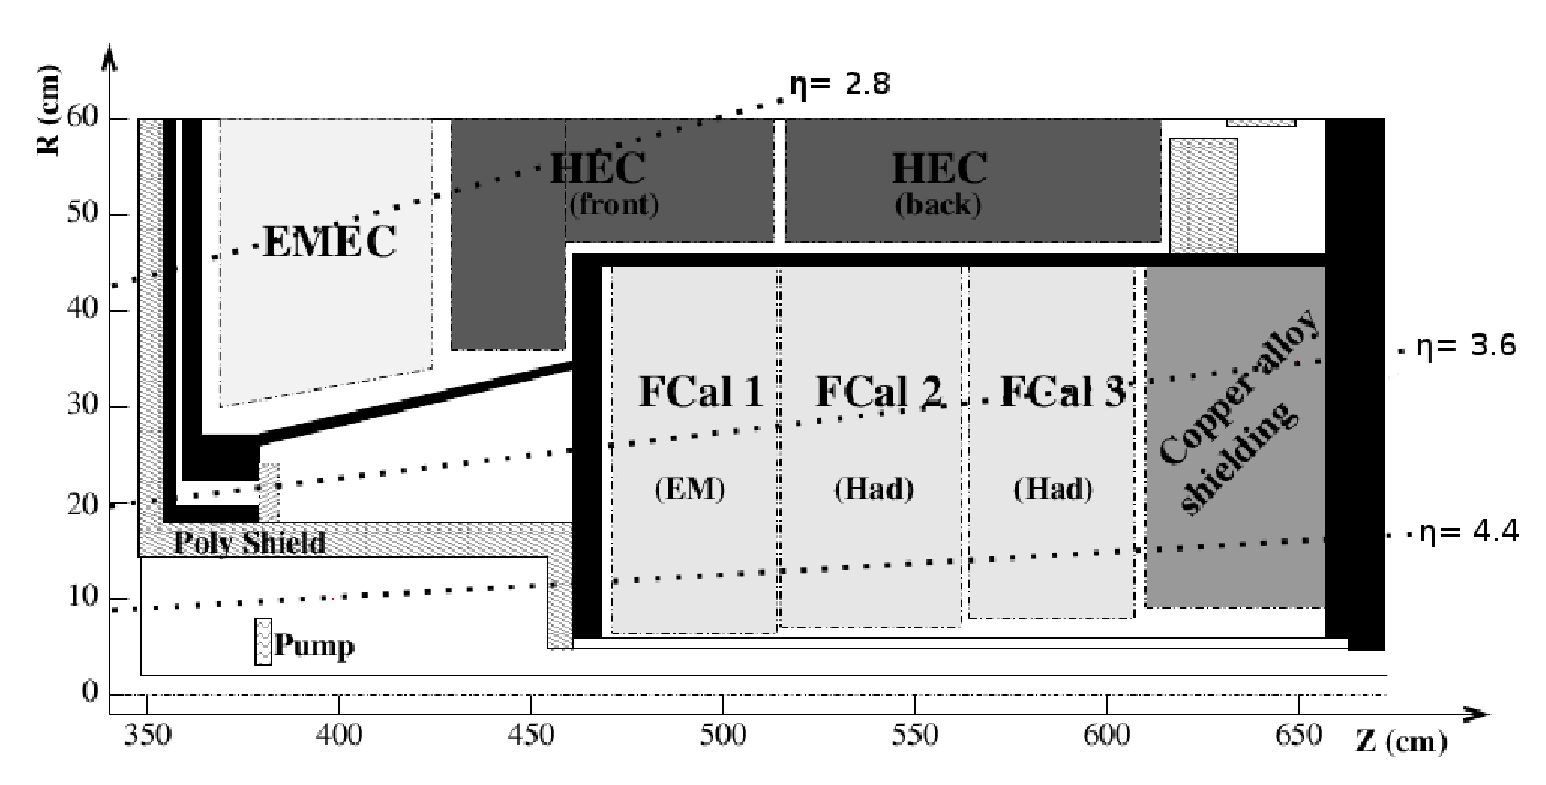
\includegraphics[width=1.0\linewidth,angle=0]{atlas_EC_xsec2.eps}\\
%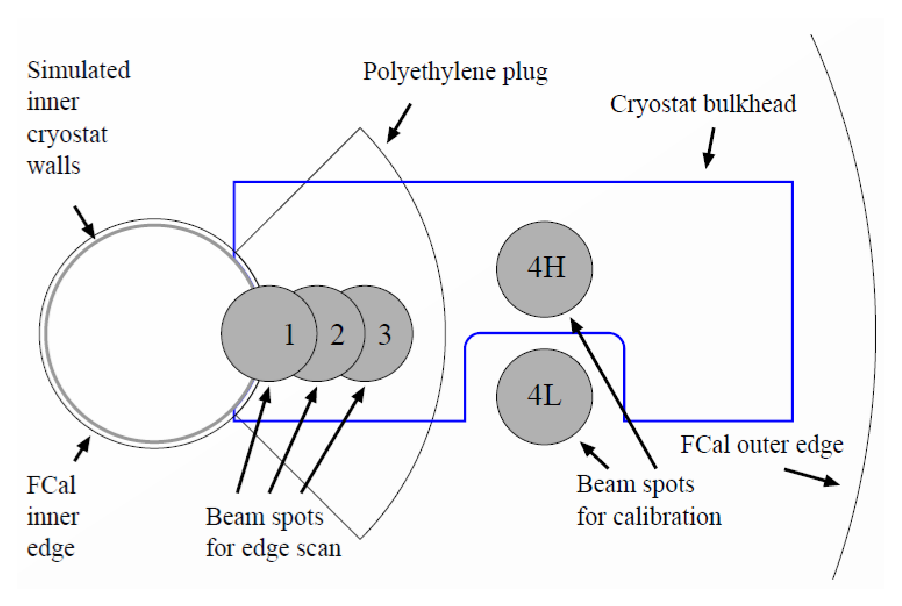
\includegraphics[width=1.0\linewidth,angle=0]{TB_beamspots.eps}\\
\end{columns}
\end{frame}
%%%%%%%%%%%%%%%%%%%%%%%%%%%%%%%%%%%%%%%%%%%%%%%%%%%%%%%%%%%%%%%%%%%

%%%%%%%%%%%%%%%%%%%%%%%%%%%%%%%%%%%%%%%%%%%%%%%%%%%%%%%%%%%%%%%%%%%
\begin{frame}\frametitle{Beamline Setup}
%\begin{columns}
%\column{0.5\linewidth}
CERN H6 Beamline
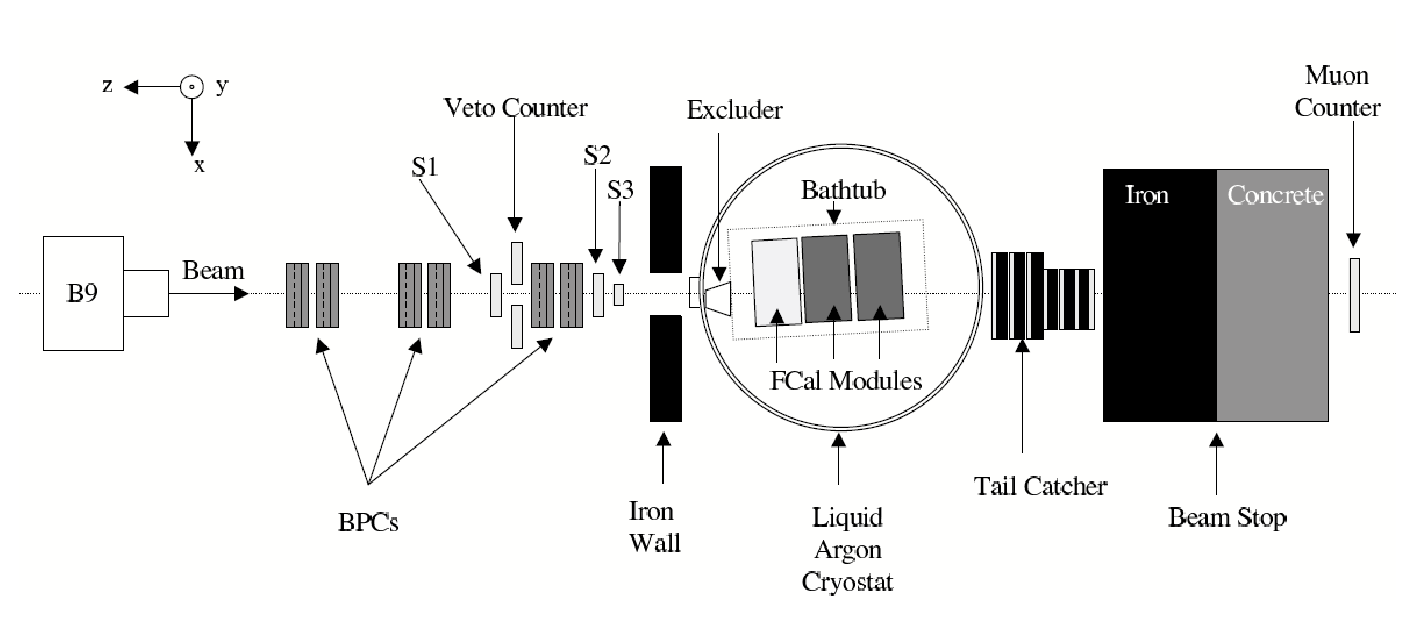
\includegraphics[width=0.8\linewidth,angle=0]{TB_Beamline.eps}
\begin{itemize}
\item Scintillators (S1,S2,S3) used for triggering.
\item BPCs (MWPCs) used to reconstruct track.
\item Both used for event selection (single particle).
\item Beam test setup modelled in \geant simulation.
\end{itemize}
%\column{0.5\linewidth}
%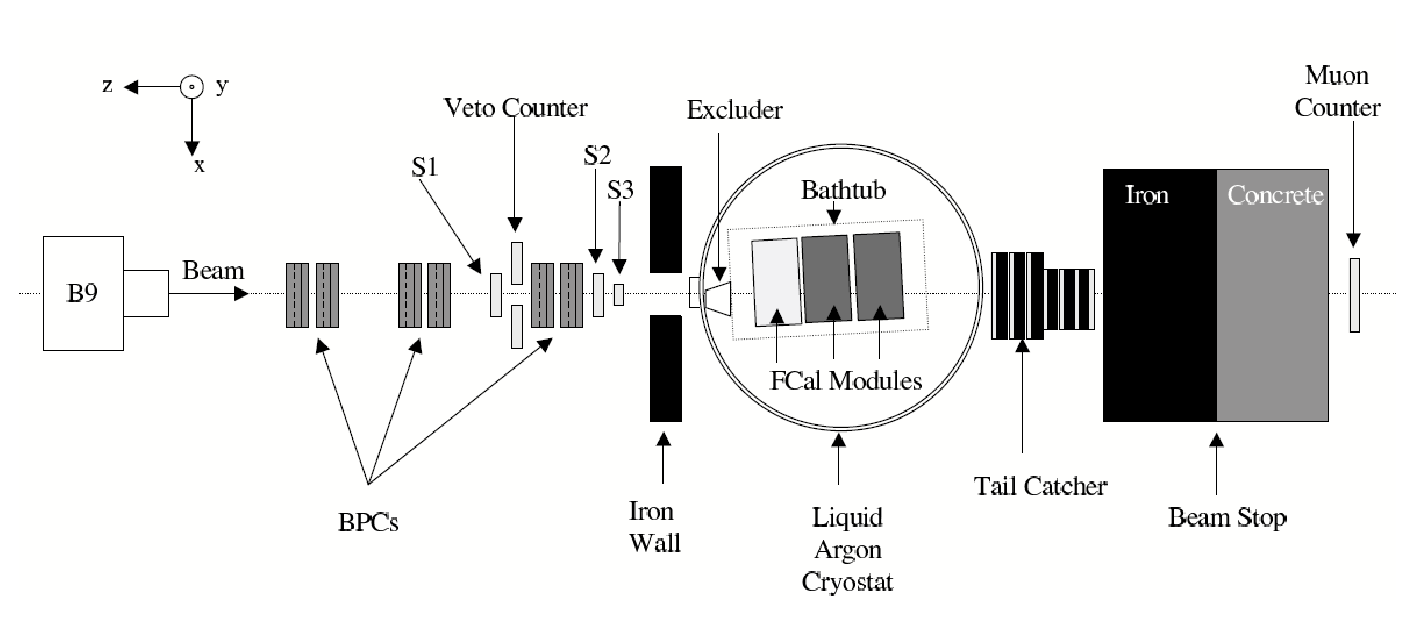
\includegraphics[width=0.8\linewidth,angle=0]{TB_Beamline.eps}
%\end{columns}
\end{frame}
%%%%%%%%%%%%%%%%%%%%%%%%%%%%%%%%%%%%%%%%%%%%%%%%%%%%%%%%%%%%%%%%%%%
%%%%%%%%%%%%%%%%%%%%%%%%%%%%%%%%%%%%%%%%%%%%%%%%%%%%%%%%%%%%%%%%%%%
\begin{frame}\frametitle{Monte Carlo Simulation}
%\begin{columns}
%\column{0.6\linewidth}
\begin{itemize}
\item Simulation of test beam developed using \geant, within \athena framework.
\begin{itemize}
\item Describes all beam elements downstream of B9 magnet.
\end{itemize}
\item Obtained results using QGSP\_BERT, QGSP\_BERT\_HP and FTFP\_BERT hadronic physics lists.
\item Electronic noise used in simulation is measured from data 
\begin{itemize}
\item Noise varied over time - different noise levels at (e.g.) different beam energies.
\item channel-channel correlations included.
\end{itemize}
\end{itemize}
\begin{columns}
\column{0.5\linewidth}
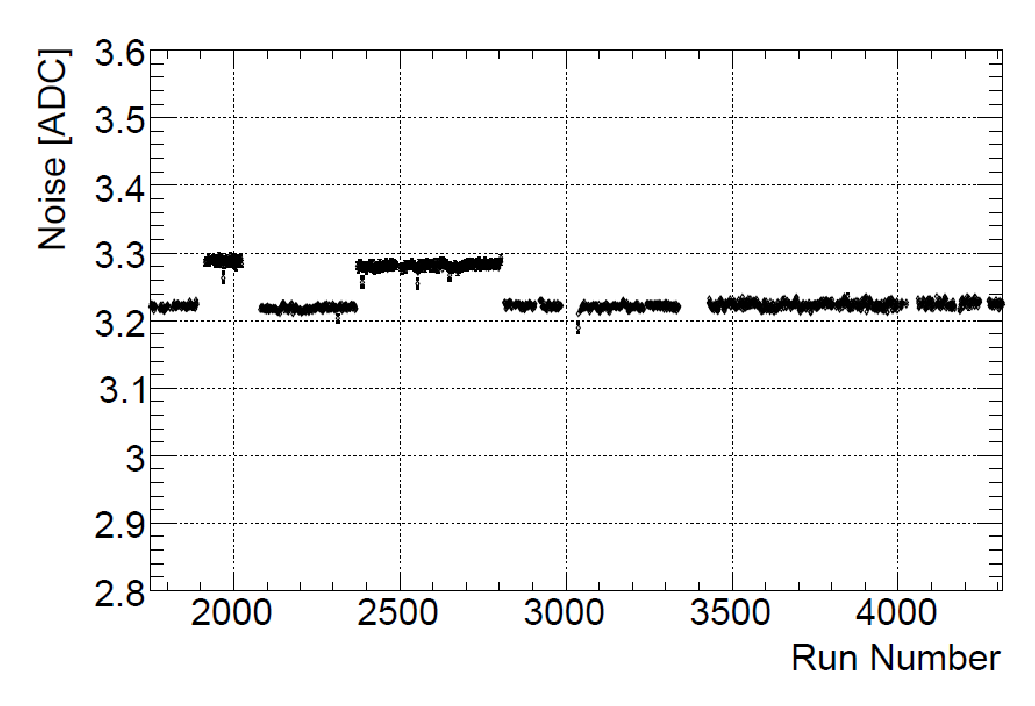
\includegraphics[width=1.0\linewidth,angle=0]{TBoverview/noise_v_run.eps}
\column{0.5\linewidth}
\blue{This effect is also accounted for in the data analysis.}
\end{columns}
\end{frame}
%%%%%%%%%%%%%%%%%%%%%%%%%%%%%%%%%%%%%%%%%%%%%%%%%%%%%%%%%%%%%%%%%%%
\begin{frame}\frametitle{Energy Reconstruction}
\begin{columns}
\column{0.6\linewidth}
\begin{itemize}
\item Reconstructed track projected to obtain particle impact point on calorimeter face.
\item Cylindrical clusters formed by summing energies of cells within radius of 8 cm (electrons) and 16 cm (hadrons).
\item Double Gaussian is fit to the peak of the response. For electron beams, hadron contamination is modelled in the fit (using hadron data). 
%\item \alert{Contribution from electronic noise to the width is measured from data.}
\end{itemize}
\column{0.4\linewidth}
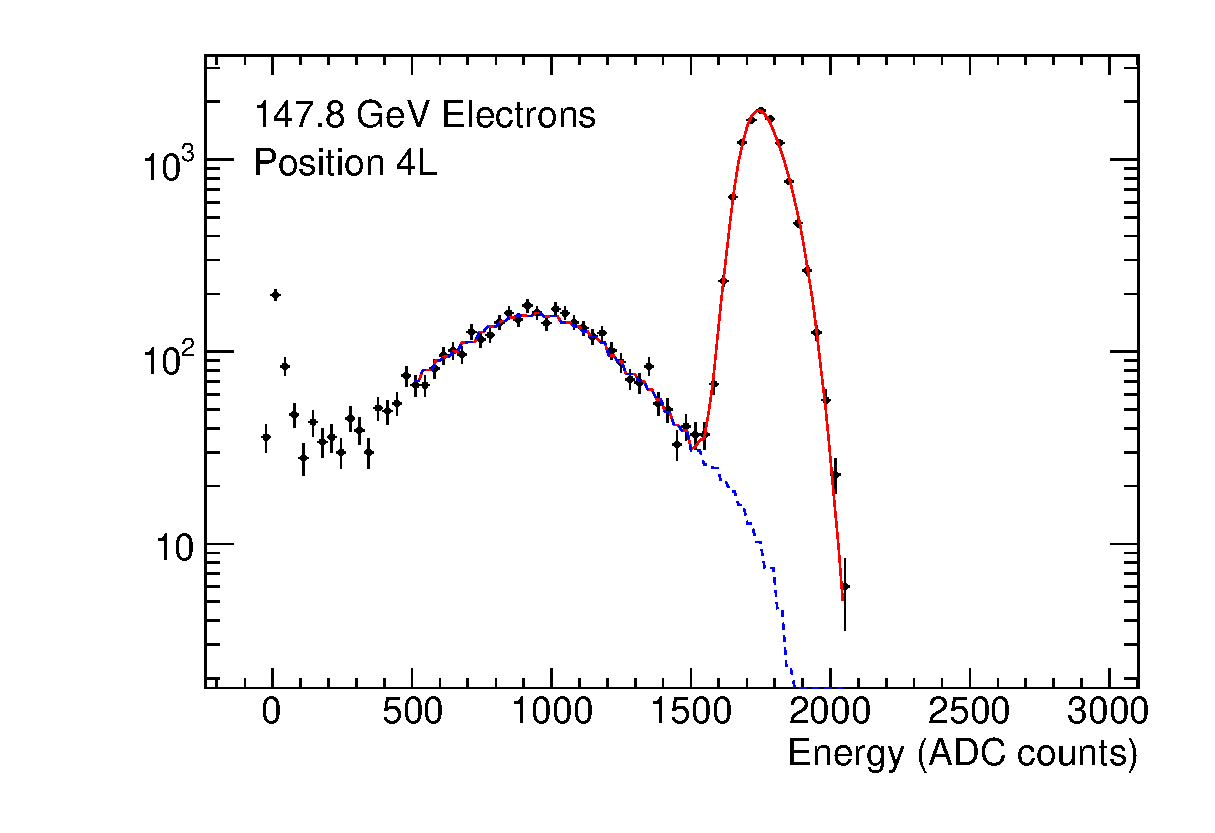
\includegraphics[width=1.0\linewidth,angle=0]{FCalTB_plots/Response_individual_data/Electron_response_148GeV_4L_data.eps}%\\
%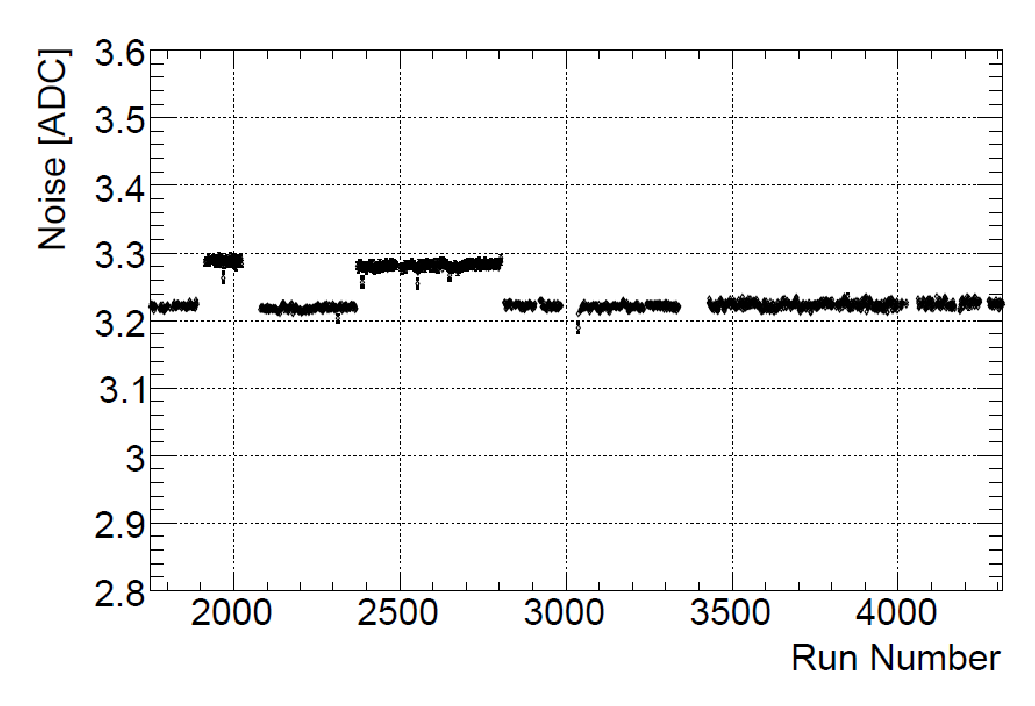
\includegraphics[width=1.0\linewidth,angle=0]{TBoverview/noise_v_run.eps}
\end{columns}
\end{frame}

%\begin{table}[htb]
%\begin{center}
%\begin{tabular}{|l|l|l|l|}
%\hline
%linearity result & slope (ADC/GeV)& Intercept (ADC) \\
%\hline
%Data (4L) & 11.966 $\pm$ 0.002 & -9.26 $\pm$ 0.07 \\
%Simulation (4L) & 11.865 $\pm$ 0.003 & -6.45 $\pm$ 0.13 \\
%Data (4H) & 11.693 $\pm$ 0.002 & -17.53 $\pm$ 0.10 \\
%Simulation (4H) & 11.747 $\pm$ 0.003 & -15.44 $\pm$ 0.13 \\
%\hline
%\end{tabular}
%\caption[Electron linearity results]{Linearity results for electron data. Quoted uncertainties are statistical.}
%\label{table_electron_c8_linearity}
%\end{center}
%\end{table}

%%%%%%%%%%%%%%%%%%%%%%%%%%%%%%%%%%%%%%%%%%%%%%%%%%%%%%%%%%%%%%%%%%%%
%\begin{frame}\frametitle{Electron Response Linearity}
%\subsection{Results}
%\begin{columns}
%\column{0.5\linewidth}
%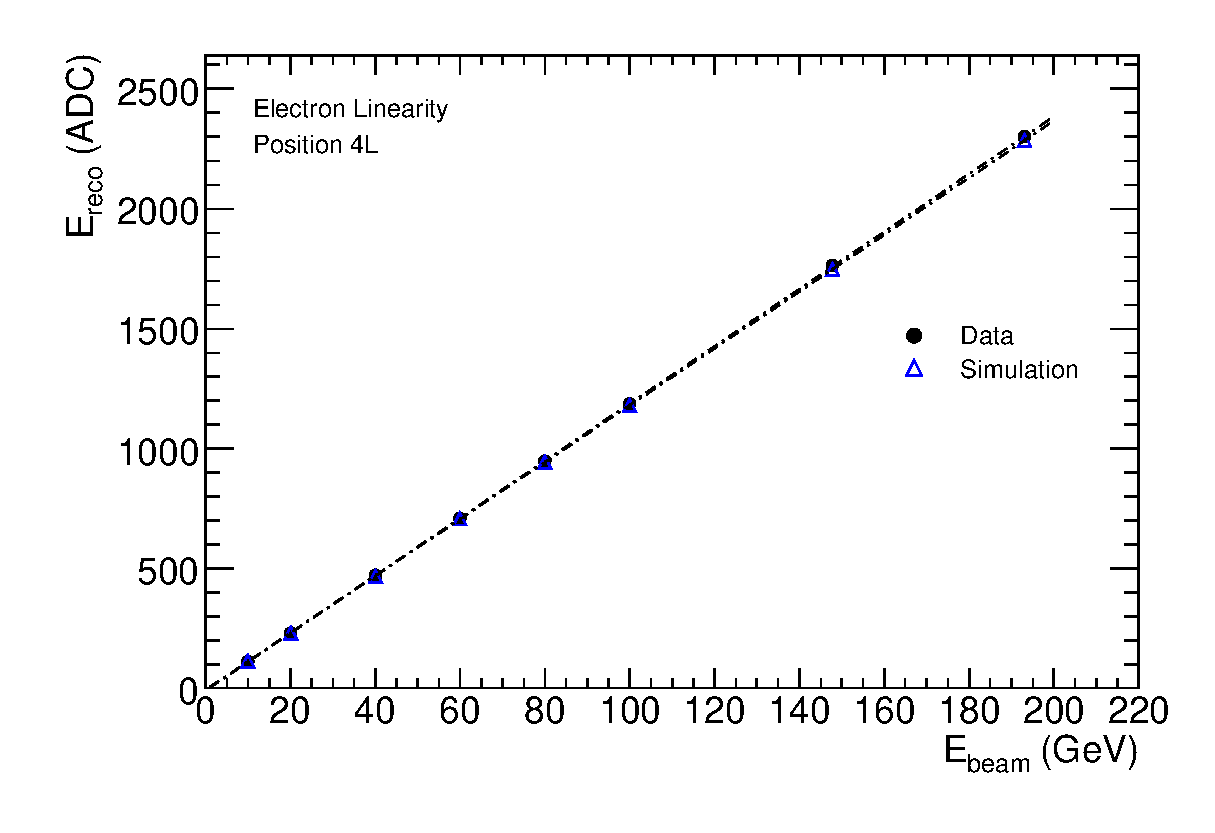
\includegraphics[width=0.95\linewidth,angle=0]{FCalTB_plots/electron_linearity_4L.eps}
%\column{0.5\linewidth}
%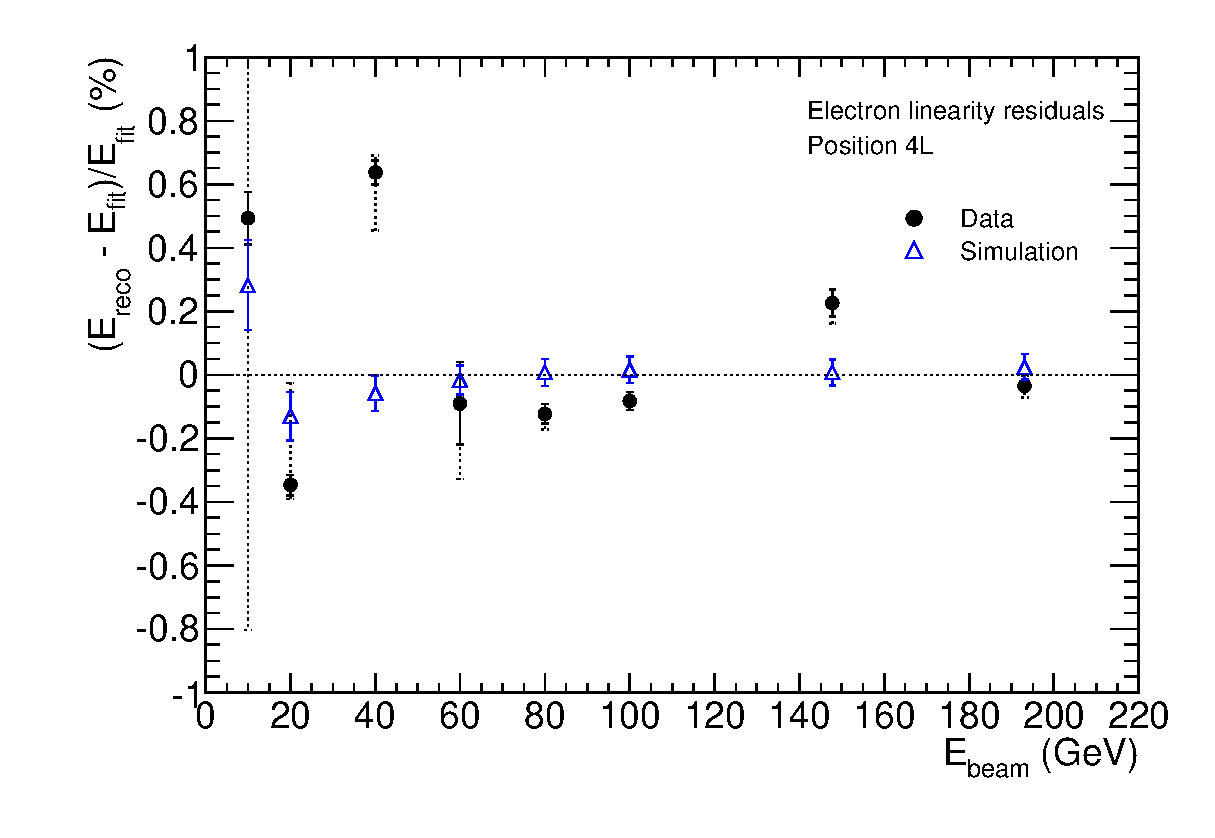
\includegraphics[width=0.95\linewidth,angle=0]{FCalTB_plots/electron_linearity_residuals_4L.eps}
%\end{columns}
%
%\begin{itemize}
%\item Response vs beam energy - expect a linear relationship. 
%\item Slope at 4L gives the EM calibration currently used at \atlas.
%\item Good agreement between Data and MC.
%\item Changes from 4L$\rightarrow$4H (not shown) similar in Data and MC.
%\end{itemize}
%%\begin{columns}
%%\column{0.4\linewidth}
%%\begin{itemize}
%%%\item Response linearity vs beam energy
%%\item Slope at position 4L consistent with prediction.
%%\item Change in intercept from 4L$\rightarrow$4H similiar in Data and MC
%%\end{itemize}
%%\column{0.6\linewidth}
%%\begin{tabular}{|l|l|l|l|}
%%\hline
%%linearity result & slope (ADC/GeV)& Intercept (ADC) \\
%%\hline
%%Data (4L) & 11.966 $\pm$ 0.002 & -9.26 $\pm$ 0.07 \\
%%Simulation (4L) & 11.865 $\pm$ 0.003 & -6.45 $\pm$ 0.13 \\
%%Data (4H) & 11.693 $\pm$ 0.002 & -17.53 $\pm$ 0.10 \\
%%Simulation (4H) & 11.747 $\pm$ 0.003 & -15.44 $\pm$ 0.13 \\
%%\hline
%%\end{tabular}
%%\end{columns}
%
%%\item Cylindrical clusters formed by summing energies of cells within radius of 8 cm (electrons) and 16 cm (hadrons).
%%\item Response is fit with a Double Gaussian (impact point dependence of response). For electron beams, hadron contamination is modelled in the fit. 
%%\end{itemize}
%%\column{0.3\linewidth}
%%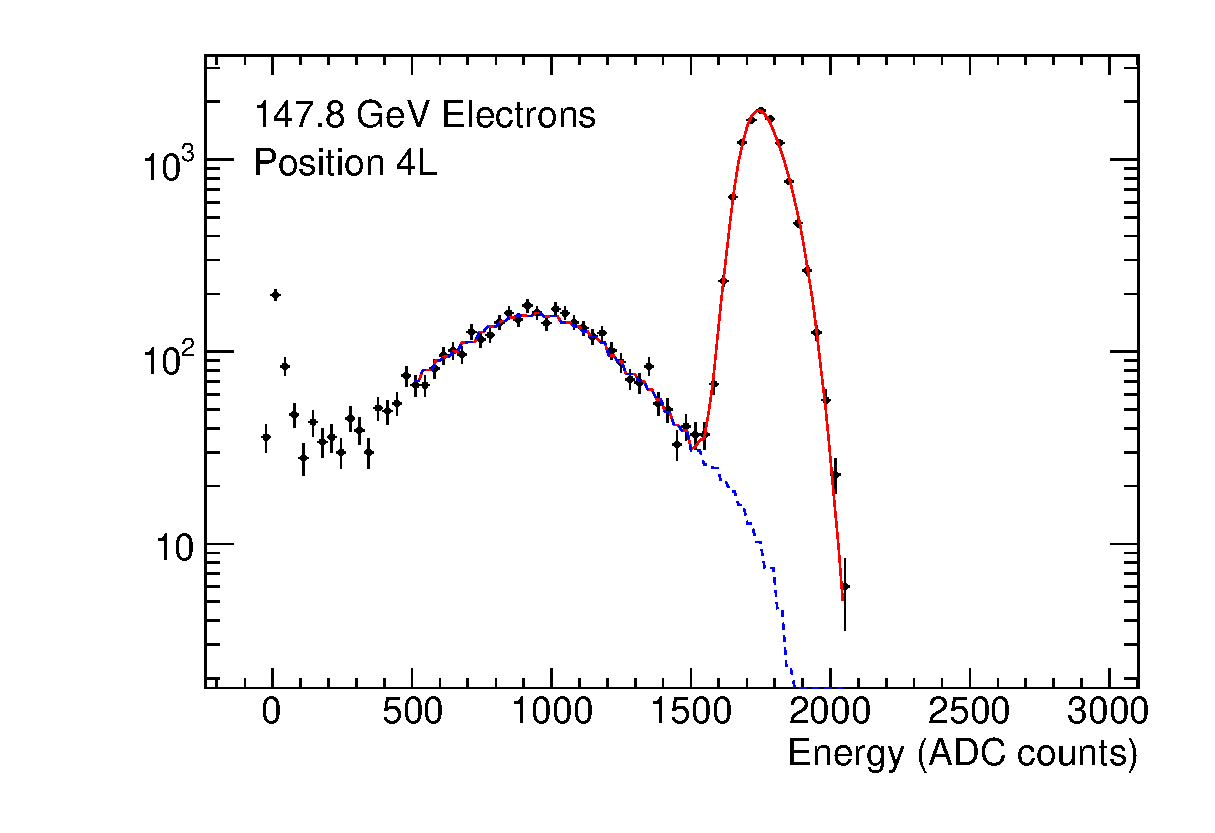
\includegraphics[width=0.8\linewidth,angle=0]{FCalTB_plots/Response_individual_data/Electron_response_148GeV_4L_data.eps}
%%\end{columns}
%\end{frame}
%
%%%%%%%%%%%%%%%%%%%%%%%%%%%%%%%%%%%%%%%%%%%%%%%%%%%%%%%%%%%%%%%%%%%%
\begin{frame}\frametitle{Electron Energy Resolution}
\begin{columns}
\column{0.5\linewidth}
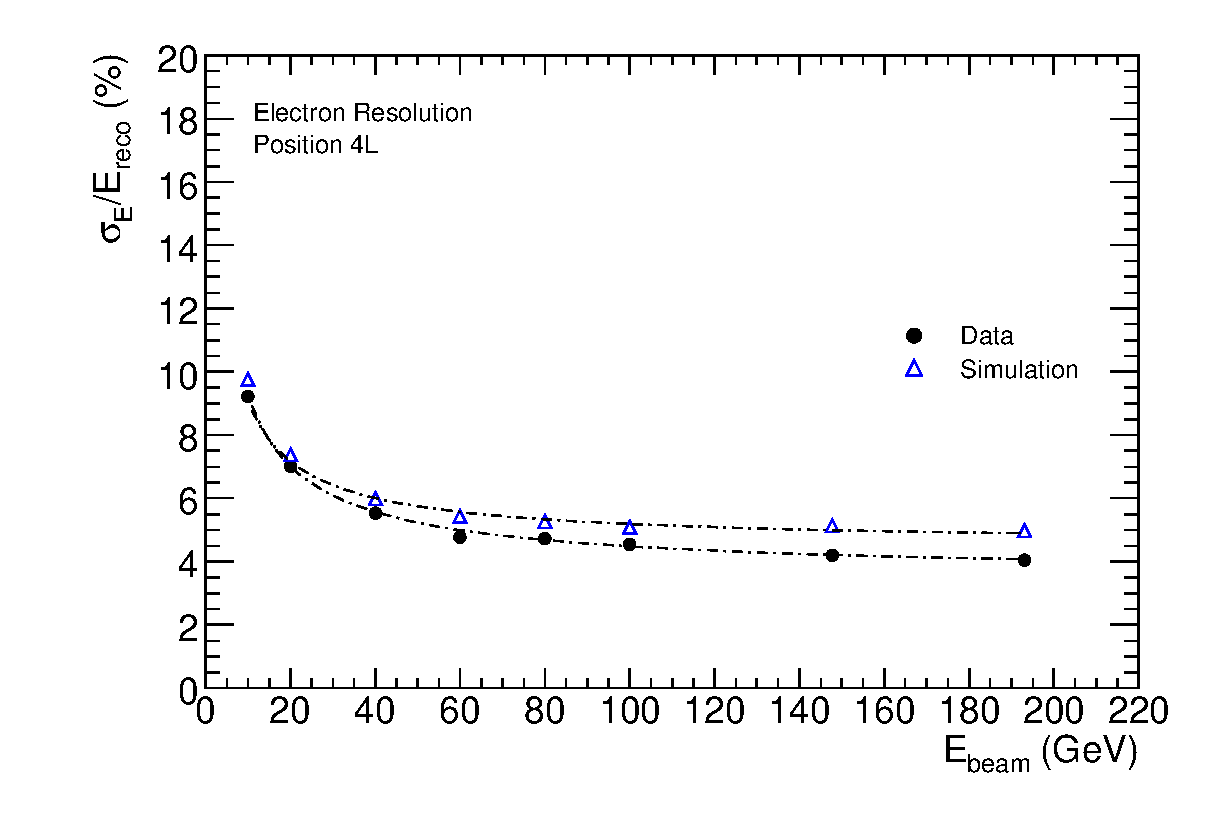
\includegraphics[width=0.95\linewidth,angle=0]{FCalTB_plots/electron_resolution_4L.eps}
\column{0.5\linewidth}
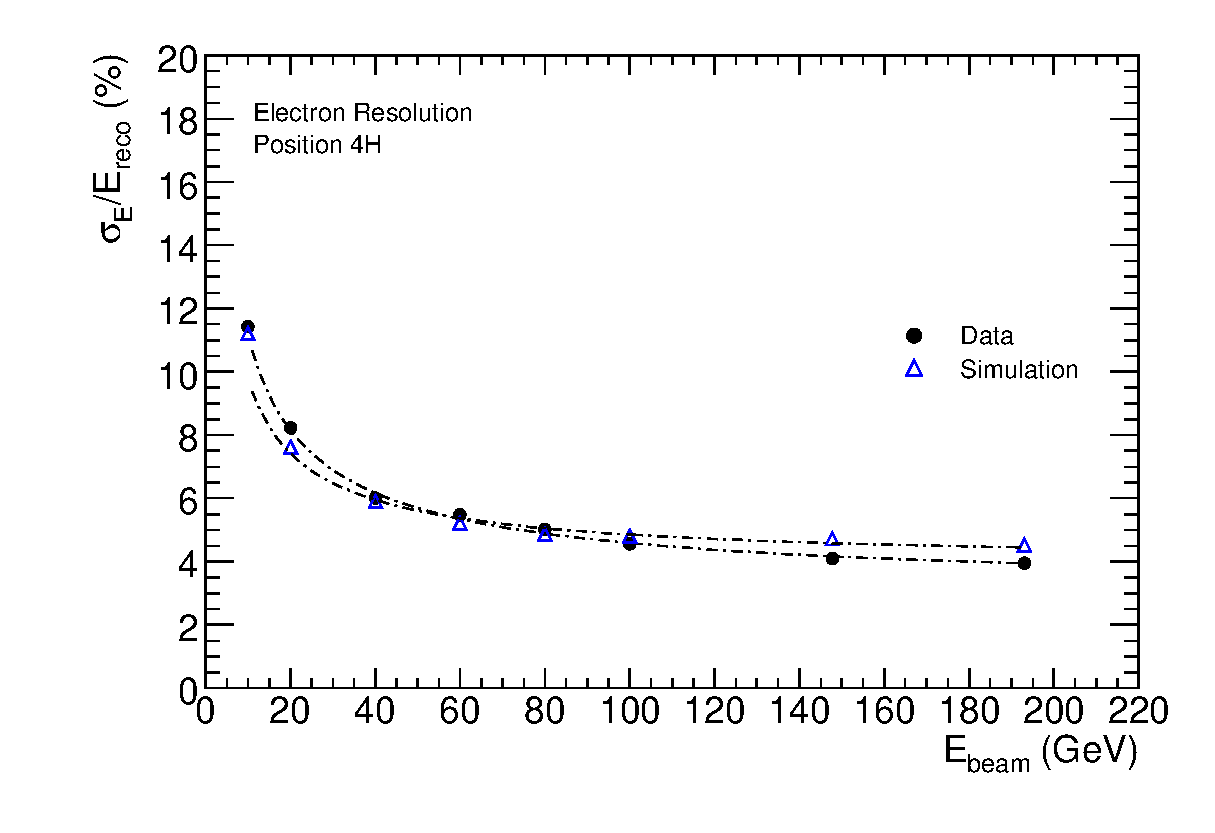
\includegraphics[width=0.95\linewidth,angle=0]{FCalTB_plots/electron_resolution_4H.eps}
\end{columns}
\begin{columns}
\column{0.5\linewidth}
\begin{equation*}
\frac{\sigma_E}{\bar{E}} = \frac{A}{\sqrt{E}} \oplus B,
\end{equation*}
\column{0.5\linewidth}
A = stochastic term\\
B = constant term
\end{columns}
\begin{itemize}
\item Resolution describes the precision with which energy can be reconstructed.
\item Noise term ($\propto 1/E$) ommitted - electronic noise subtracted in quadrature from width.
\item Resolution in simulation slightly higher (worse) than in data - consistent with other \geant results.
\item Constant term at 4L 15\% higher than 4H, in both data and MC.
\end{itemize}
%\column{0.3\linewidth}
%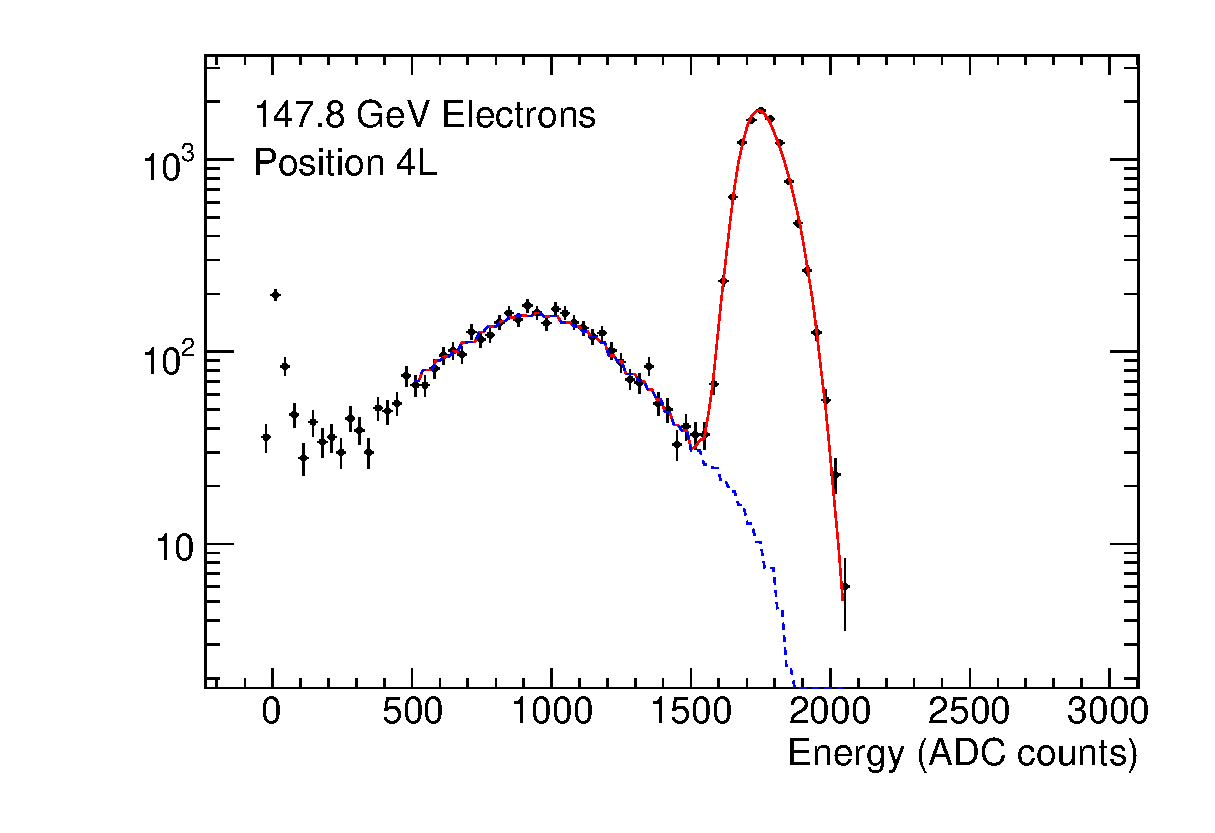
\includegraphics[width=0.8\linewidth,angle=0]{FCalTB_plots/Response_individual_data/Electron_response_148GeV_4L_data.eps}
%\end{columns}
\end{frame}
%%%%%%%%%%%%%%%%%%%%%%%%%%%%%%%%%%%%%%%%%%%%%%%%%%%%%%%%%%%%%%%%%%%
%\begin{frame}\frametitle{Hadronic Calibration}
%\begin{columns}
%\column{0.5\linewidth}
%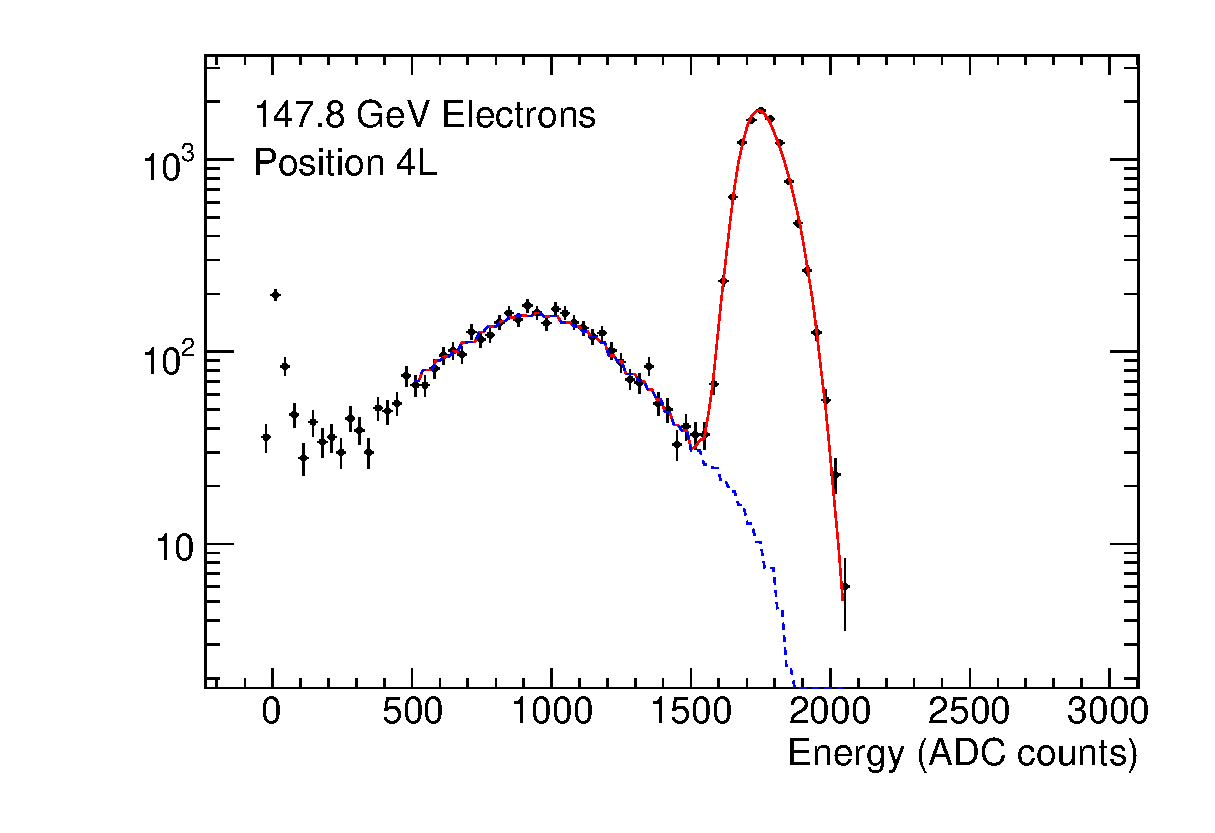
\includegraphics[width=0.8\linewidth,angle=0]{FCalTB_plots/Response_individual_data/Electron_response_148GeV_4L_data.eps}
%\column{0.5\linewidth}
%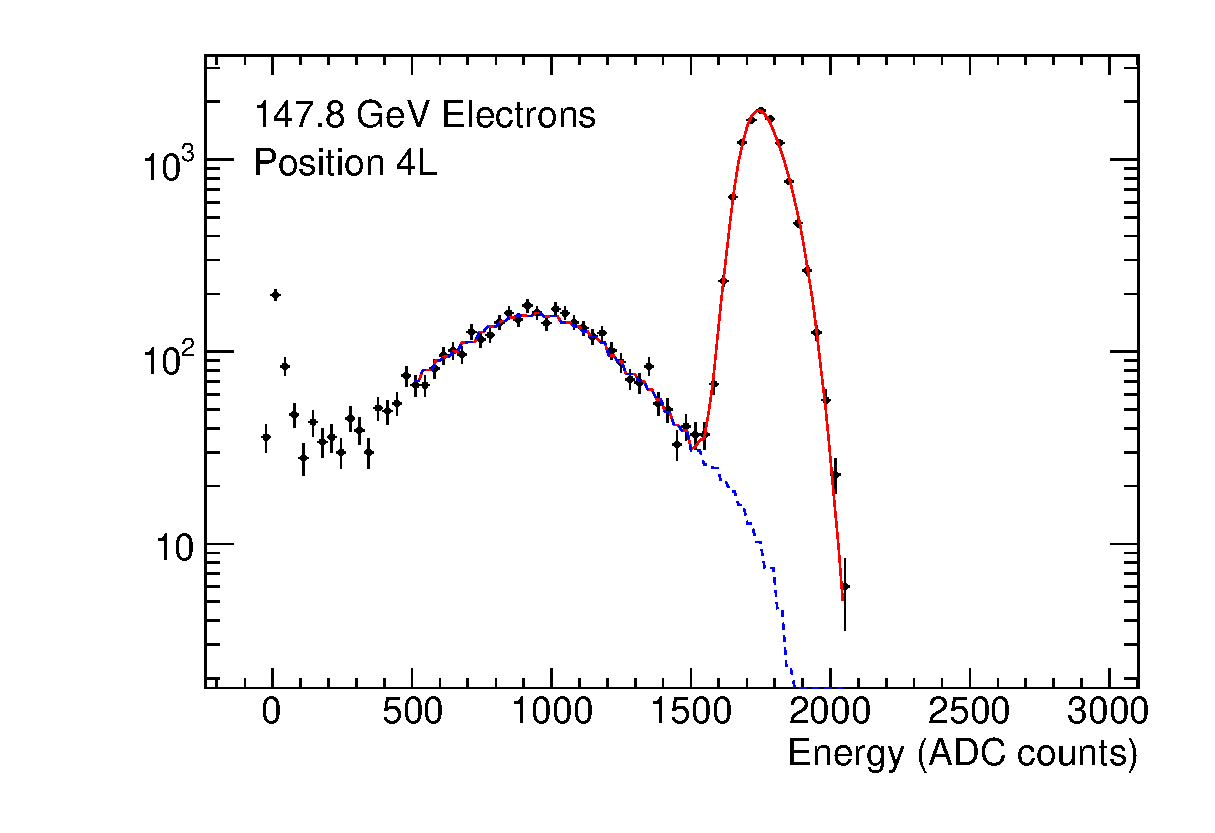
\includegraphics[width=0.8\linewidth,angle=0]{FCalTB_plots/Response_individual_data/Electron_response_148GeV_4L_data.eps}
%\end{columns}
%\begin{itemize}
%\item resolution results and numbers
%\item Cylindrical clusters formed by summing energies of cells within radius of 8 cm (electrons) and 16 cm (hadrons).
%\item Response is fit with a Double Gaussian (impact point dependence of response). For electron beams, hadron contamination is modelled in the fit. 
%\end{itemize}
%%\column{0.3\linewidth}
%%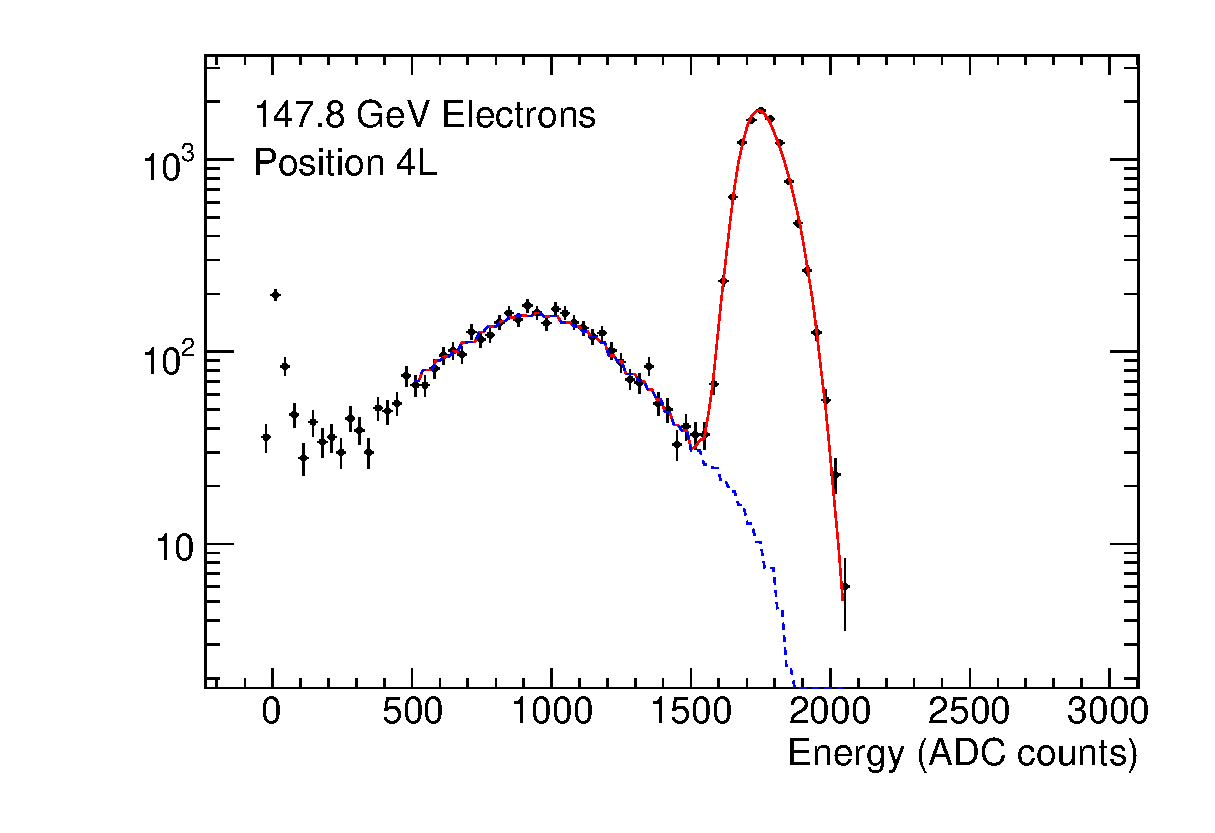
\includegraphics[width=0.8\linewidth,angle=0]{FCalTB_plots/Response_individual_data/Electron_response_148GeV_4L_data.eps}
%%\end{columns}
%\end{frame}
%%%%%%%%%%%%%%%%%%%%%%%%%%%%%%%%%%%%%%%%%%%%%%%%%%%%%%%%%%%%%%%%%%%
\begin{frame}\frametitle{Pion Response}
\begin{columns}
\column{0.5\linewidth}
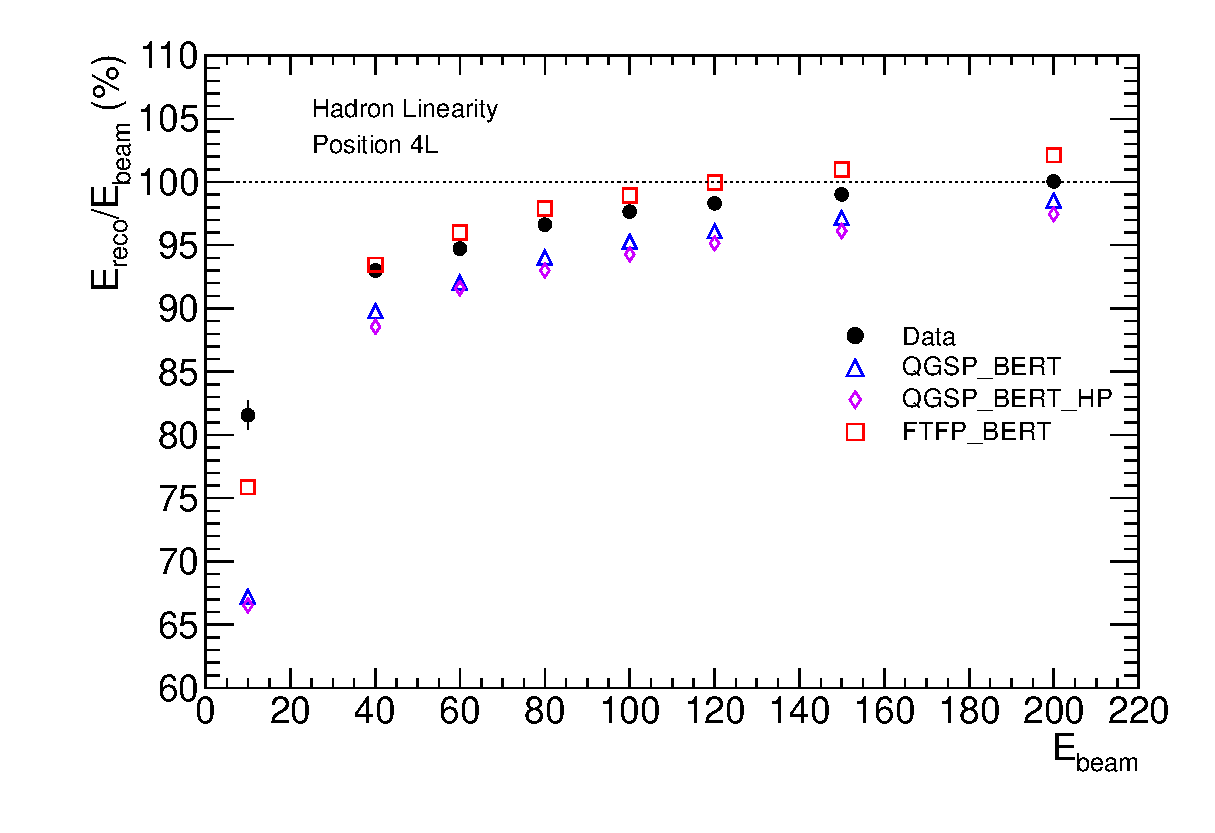
\includegraphics[width=0.95\linewidth,angle=0]{FCalTB_plots/hadron_linearity_4L.eps}
\column{0.5\linewidth}
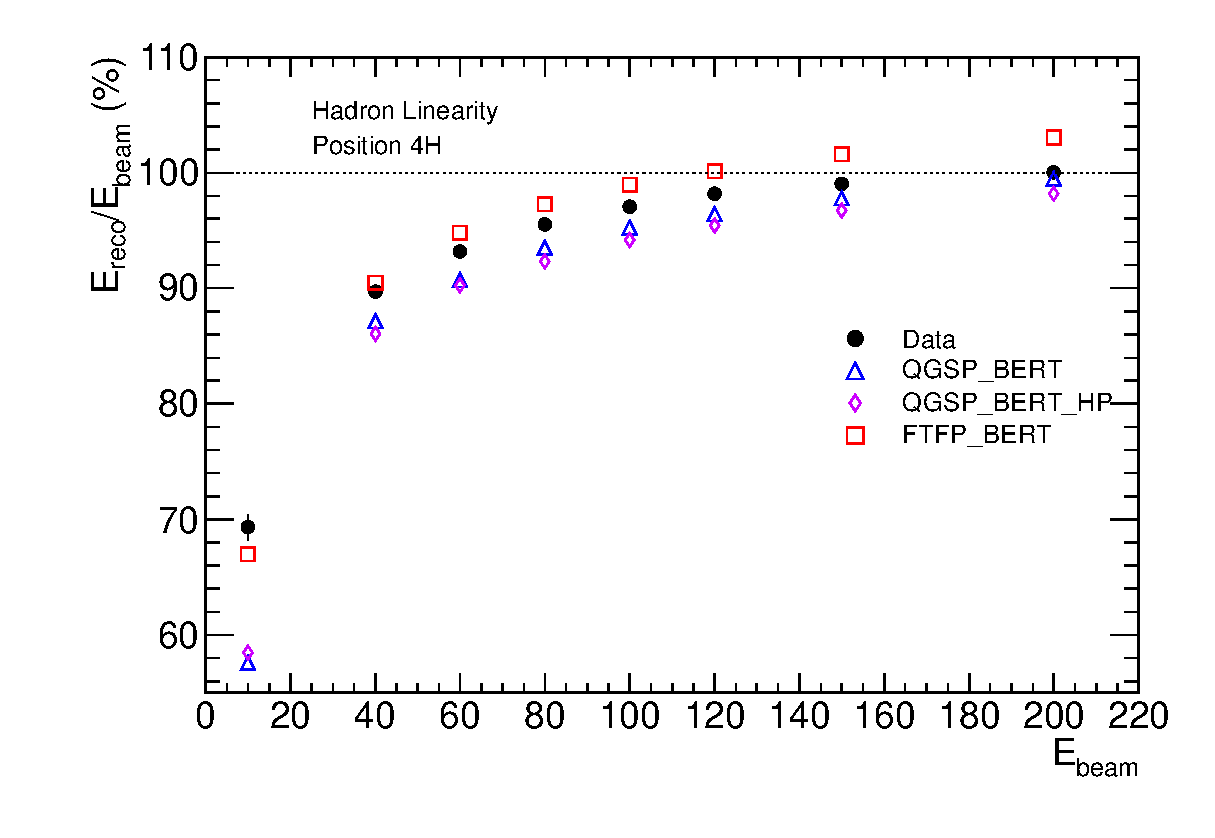
\includegraphics[width=0.95\linewidth,angle=0]{FCalTB_plots/hadron_linearity_4H.eps}
\end{columns}
\begin{itemize}
\item Pions deposit less visible energy in the calorimeter - require calibration.
\item Simple flat weighting scheme used for hadronic calibration - each module has a weight associated with it.
\begin{equation*}
E_\mathrm{cal} = g_1 E_{1,\mathrm{EM}} +g_2 E_{2,\mathrm{EM}} +g_3 E_{3,\mathrm{EM}}
\end{equation*}
\item Weights derived from 200 GeV data used to calibrate data and MC.
\item MC results generally within a few percent of data.
%\item Different physics lists studied - use different models for hadronic interactions.
%\item 
\end{itemize}
%\column{0.3\linewidth}
%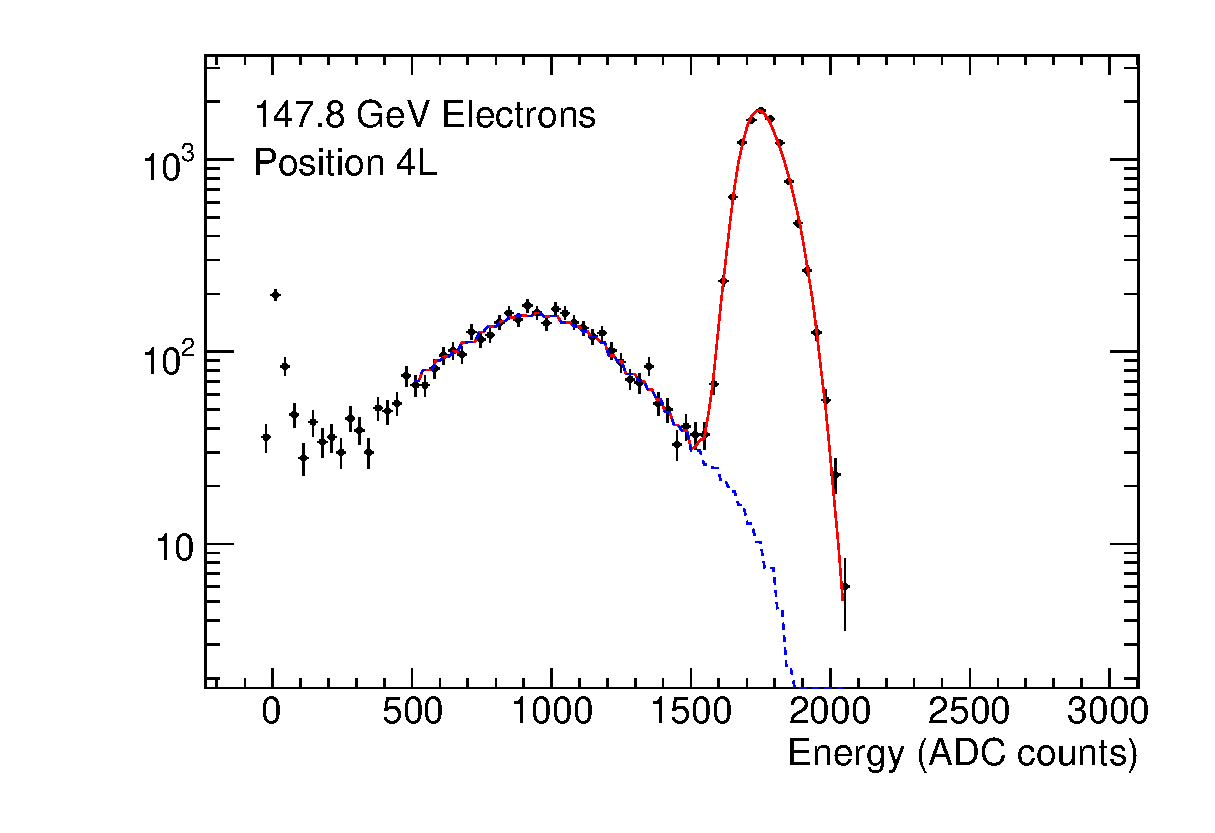
\includegraphics[width=0.8\linewidth,angle=0]{FCalTB_plots/Response_individual_data/Electron_response_148GeV_4L_data.eps}
%\end{columns}
\end{frame}
%%%%%%%%%%%%%%%%%%%%%%%%%%%%%%%%%%%%%%%%%%%%%%%%%%%%%%%%%%%%%%%%%%%
\begin{frame}\frametitle{Pion Resolution}
\begin{columns}
\column{0.5\linewidth}
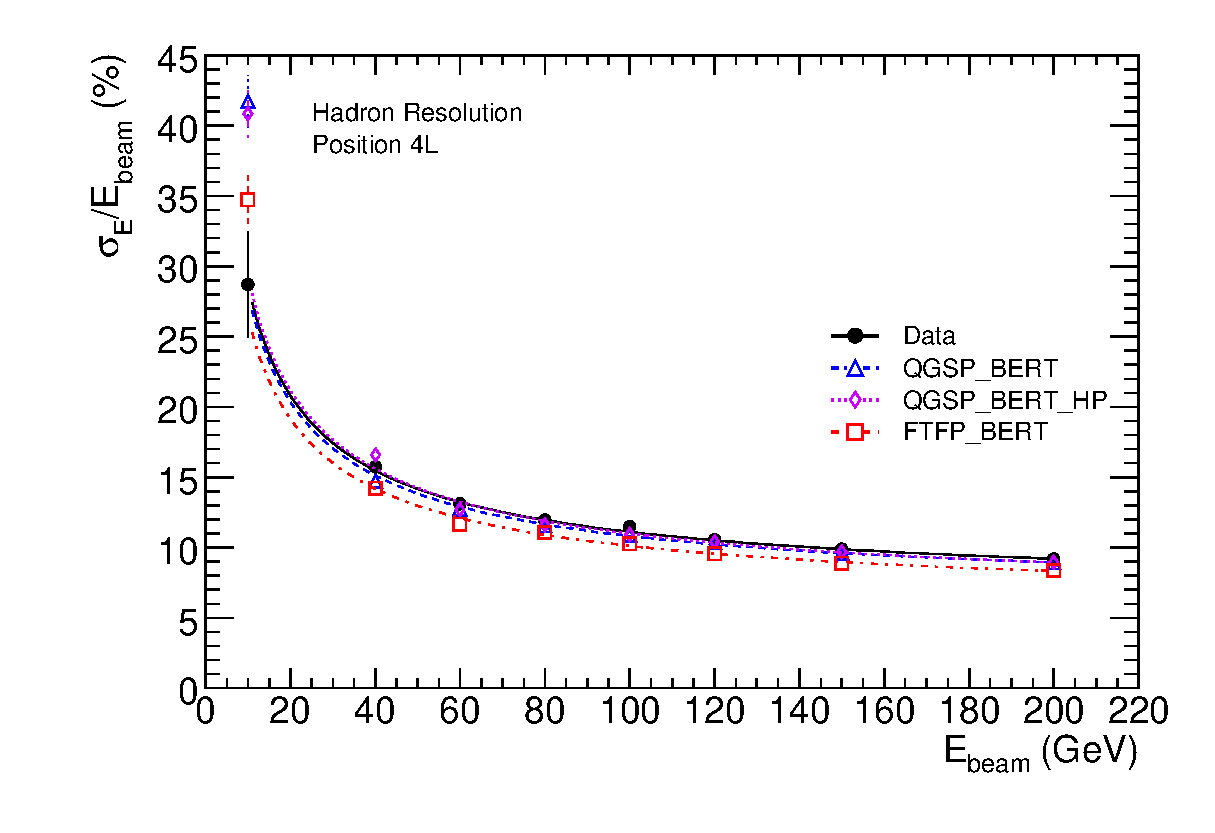
\includegraphics[width=0.95\linewidth,angle=0]{FCalTB_plots/hadron_resolution_4L.eps}
\column{0.5\linewidth}
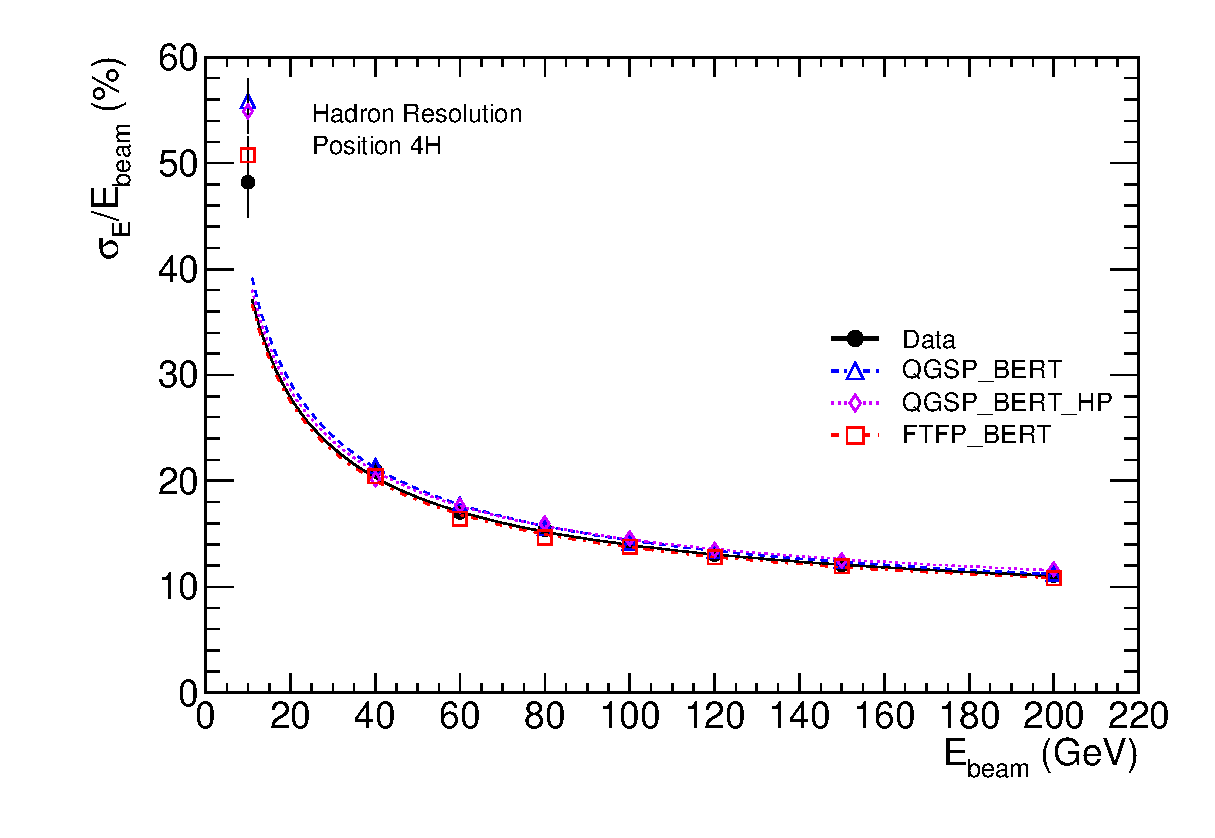
\includegraphics[width=0.95\linewidth,angle=0]{FCalTB_plots/hadron_resolution_4H.eps}
\end{columns}
\begin{itemize}
%\item Resolution describes the precision with which energy can be reconstructed.
\item Resolution at 4L slightly improved compared to previously published result (corrected energy rounding bug).
\item Generally good agreement between Data and MC.
\item Changes from 4L$\rightarrow$4H similar in Data and MC.
\begin{itemize}
\item Effects of additional material are well modelled by the simulation.
\end{itemize}
\end{itemize}
%\column{0.3\linewidth}
%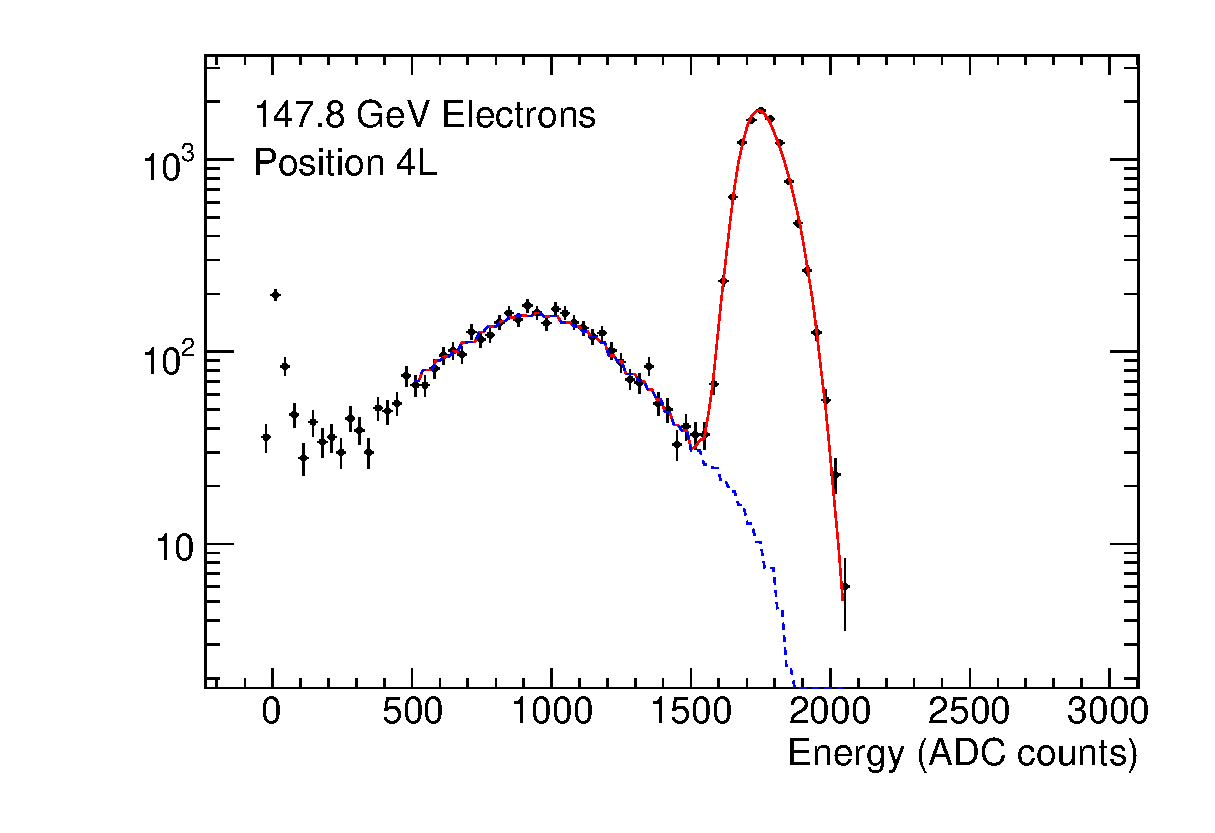
\includegraphics[width=0.8\linewidth,angle=0]{FCalTB_plots/Response_individual_data/Electron_response_148GeV_4L_data.eps}
%\end{columns}
\end{frame}
%%%%%%%%%%%%%%%%%%%%%%%%%%%%%%%%%%%%%%%%%%%%%%%%%%%%%%%%%%%%%%%%%%%
\begin{frame}\frametitle{Testbeam summary}
\begin{itemize}
\item Analysed data at 4L and 4H - response and resolution of the FCal have been measured using beams of electrons and hadrons at energies of 10-200 GeV.
\item Simulation agrees well with data - Changes from 4L $\rightarrow$ 4H well modelled by simulation.
\item Validation of MC for the FCal, important as all \atlas hadronic calibrations are derived from MC.
\item Shower shapes and topological clusters have also been studied.
\end{itemize}
\end{frame}
%%%%%%%%%%%%%%%%%%%%%%%%%%%%%%%%%%%%%%%%%%%%%%%%%%%%%%%%%%%%%%%%%%%
%\begin{frame}\frametitle{Cluster Moments}
%\begin{columns}
%\column{0.5\linewidth}
%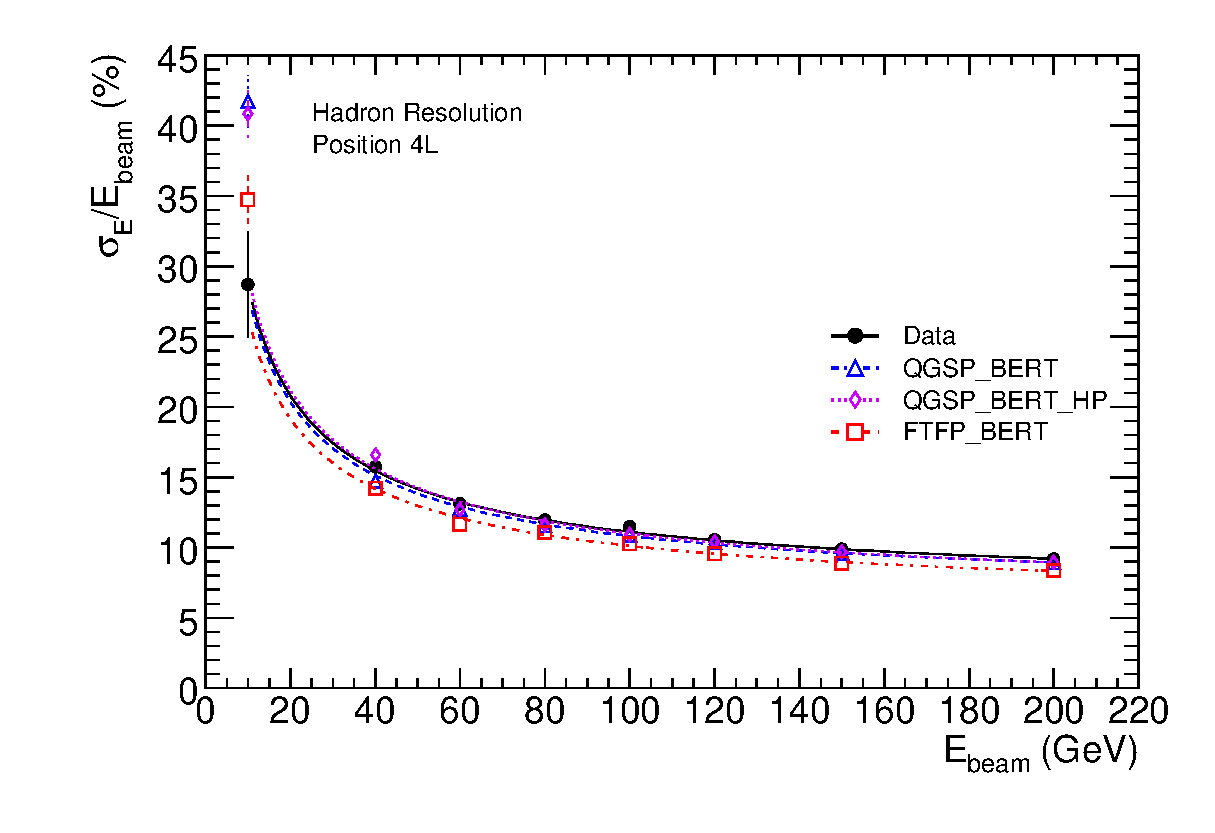
\includegraphics[width=0.8\linewidth,angle=0]{FCalTB_plots/hadron_resolution_4L.eps}
%\column{0.5\linewidth}
%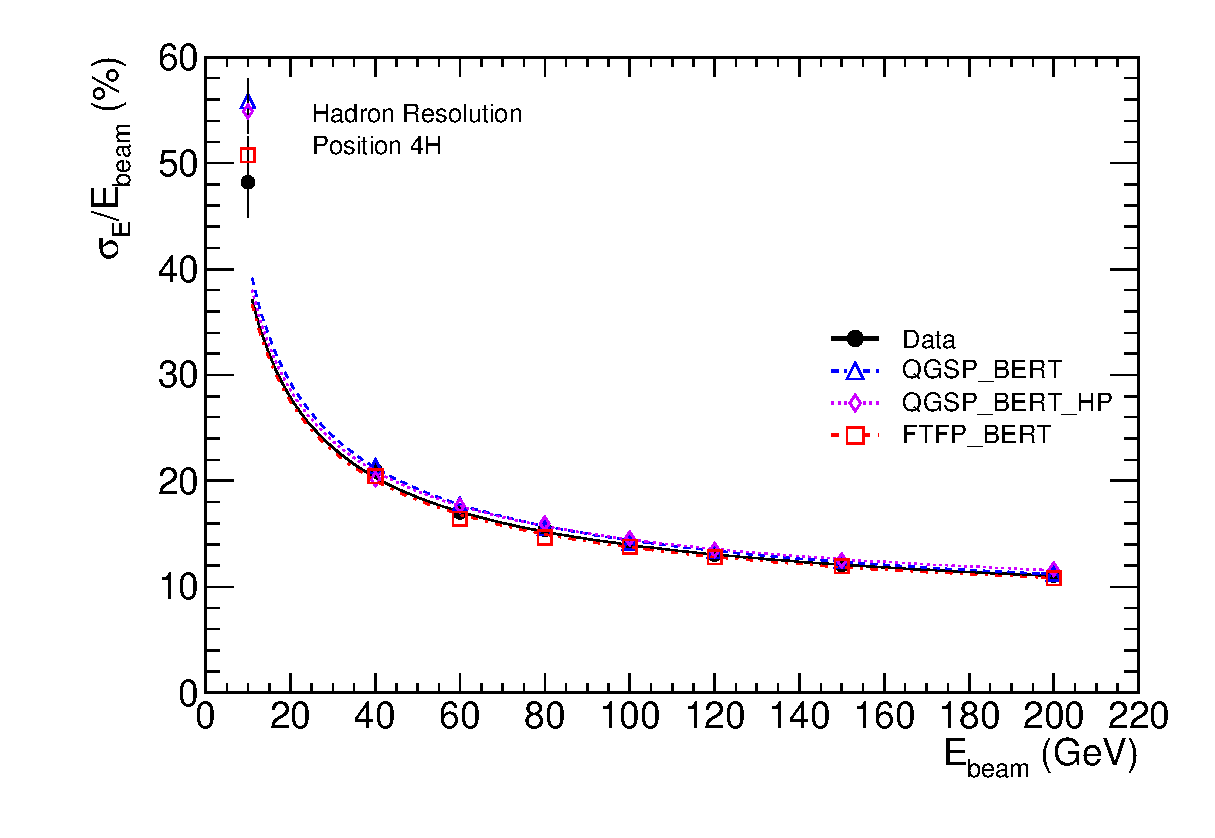
\includegraphics[width=0.8\linewidth,angle=0]{FCalTB_plots/hadron_resolution_4H.eps}
%\end{columns}
%\begin{itemize}
%\item Hadronic calibration - flat weights.
%\item Weights from MC generally agree with those from data.
%\item Weights derived from data at 200 GeV are used to reconstruct (most) data and MC results.
%\end{itemize}
%%\column{0.3\linewidth}
%%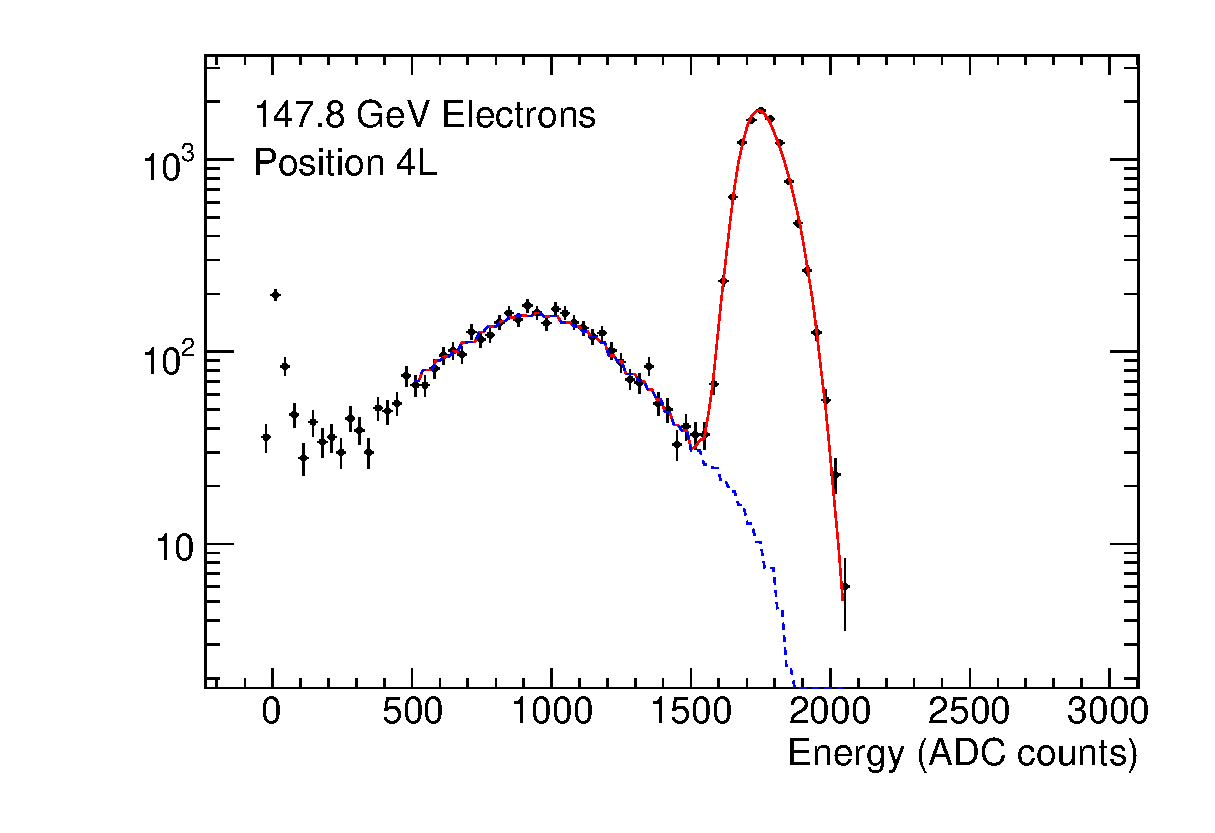
\includegraphics[width=0.8\linewidth,angle=0]{FCalTB_plots/Response_individual_data/Electron_response_148GeV_4L_data.eps}
%%\end{columns}
%\end{frame}
%%%%%%%%%%%%%%%%%%%%%%%%%%%%%%%%%%%%%%%%%%%%%%%%%%%%%%%%%%%%%%%%%%%%
%\begin{frame}\frametitle{Cluster Moments}
%\begin{columns}
%\column{0.5\linewidth}
%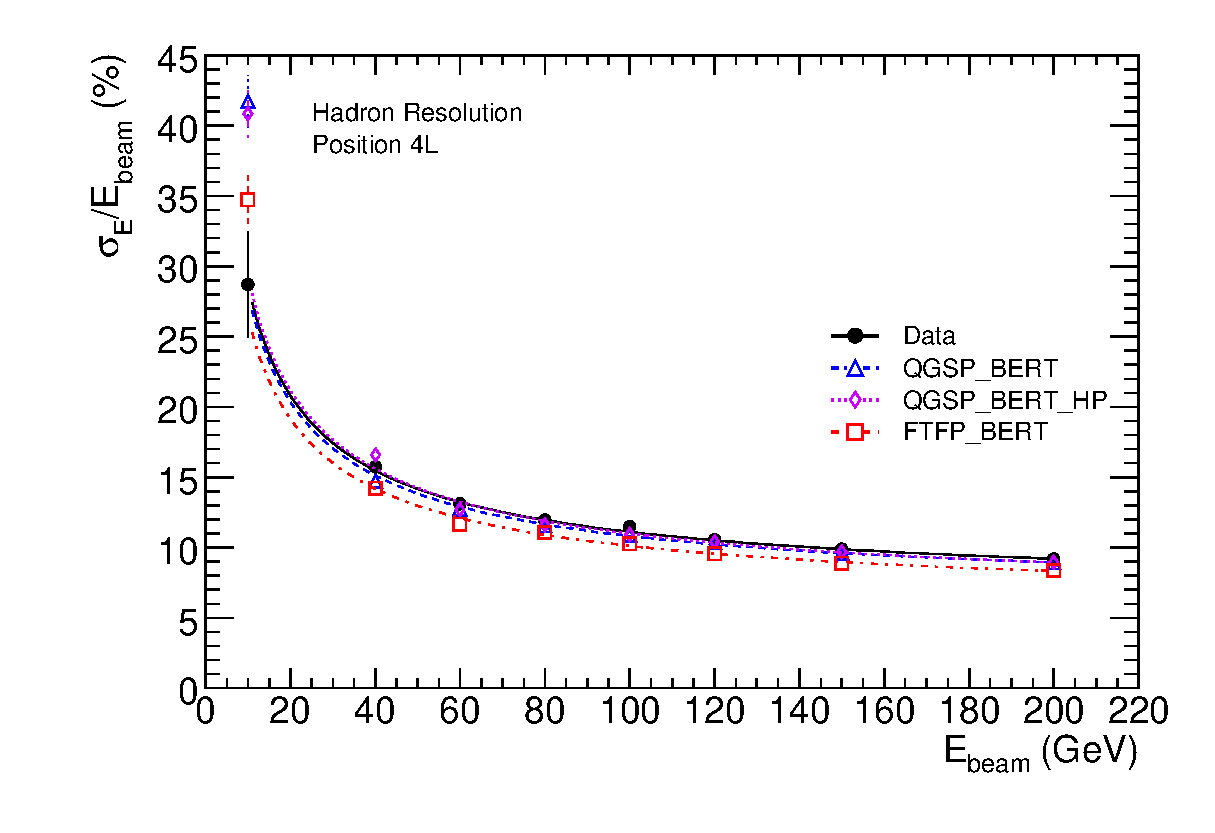
\includegraphics[width=0.8\linewidth,angle=0]{FCalTB_plots/hadron_resolution_4L.eps}
%\column{0.5\linewidth}
%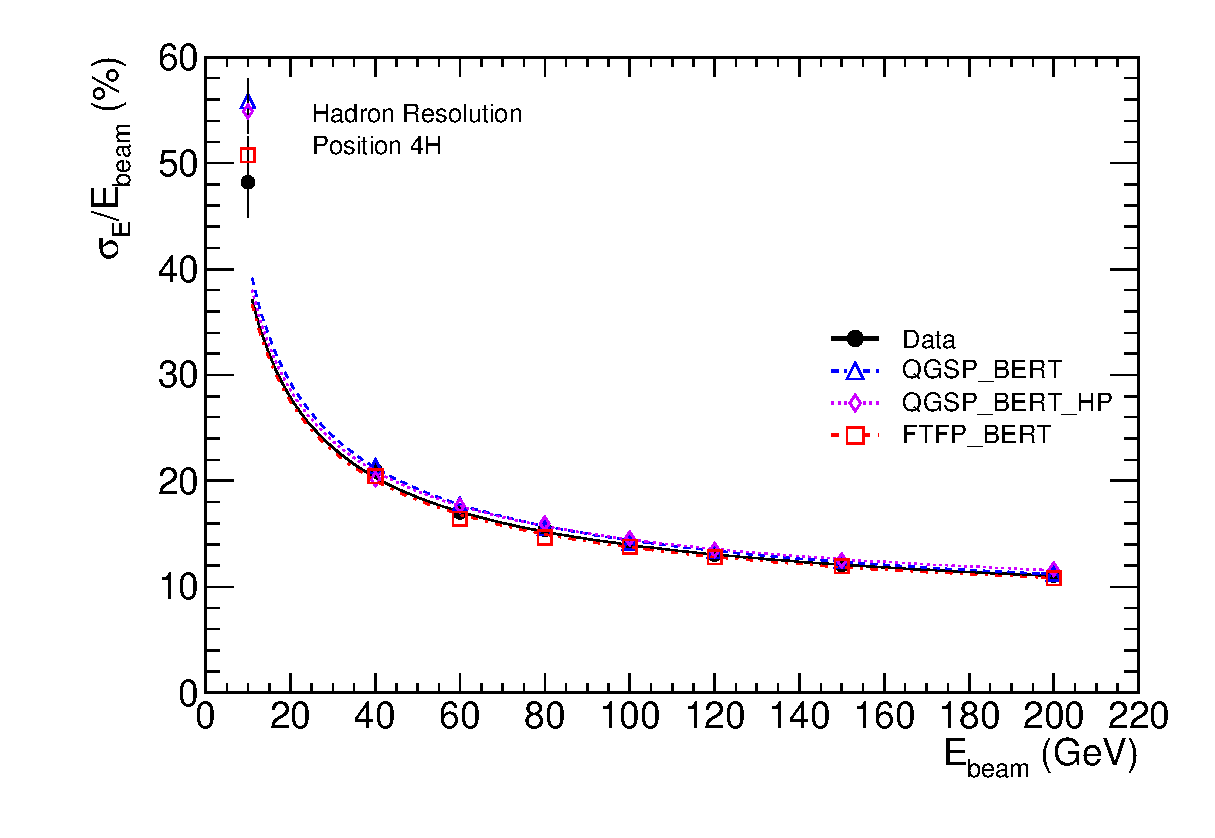
\includegraphics[width=0.8\linewidth,angle=0]{FCalTB_plots/hadron_resolution_4H.eps}
%\end{columns}
%\begin{itemize}
%\item Hadronic calibration - flat weights.
%\item Weights from MC generally agree with those from data.
%\item Weights derived from data at 200 GeV are used to reconstruct (most) data and MC results.
%\end{itemize}
%%\column{0.3\linewidth}
%%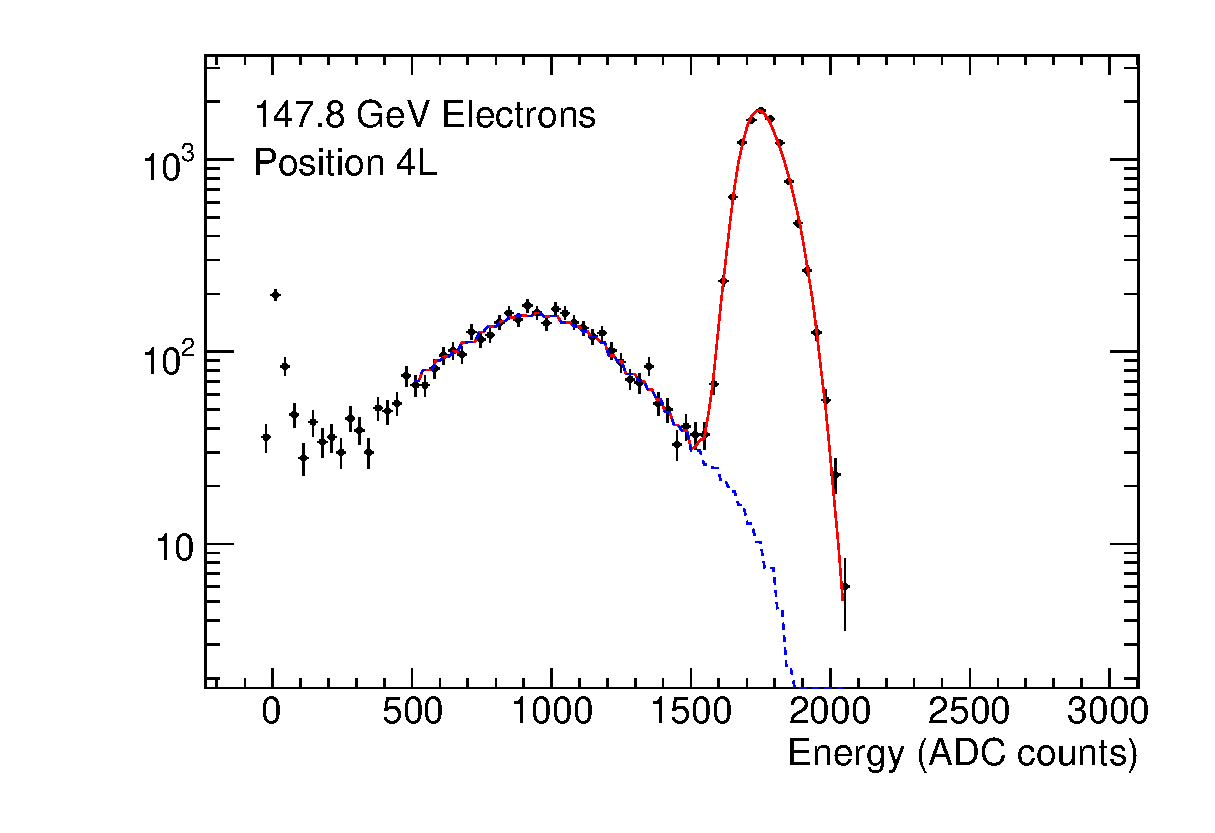
\includegraphics[width=0.8\linewidth,angle=0]{FCalTB_plots/Response_individual_data/Electron_response_148GeV_4L_data.eps}
%%\end{columns}
%\end{frame}
%%%%%%%%%%%%%%%%%%%%%%%%%%%%%%%%%%%%%%%%%%%%%%%%%%%%%%%%%%%%%%%%%%%
\section{Inclusive Jet Cross-Section}
\begin{frame}\frametitle{Inclusive Jet Cross-Section}
\begin{columns}
\column{0.6\linewidth}
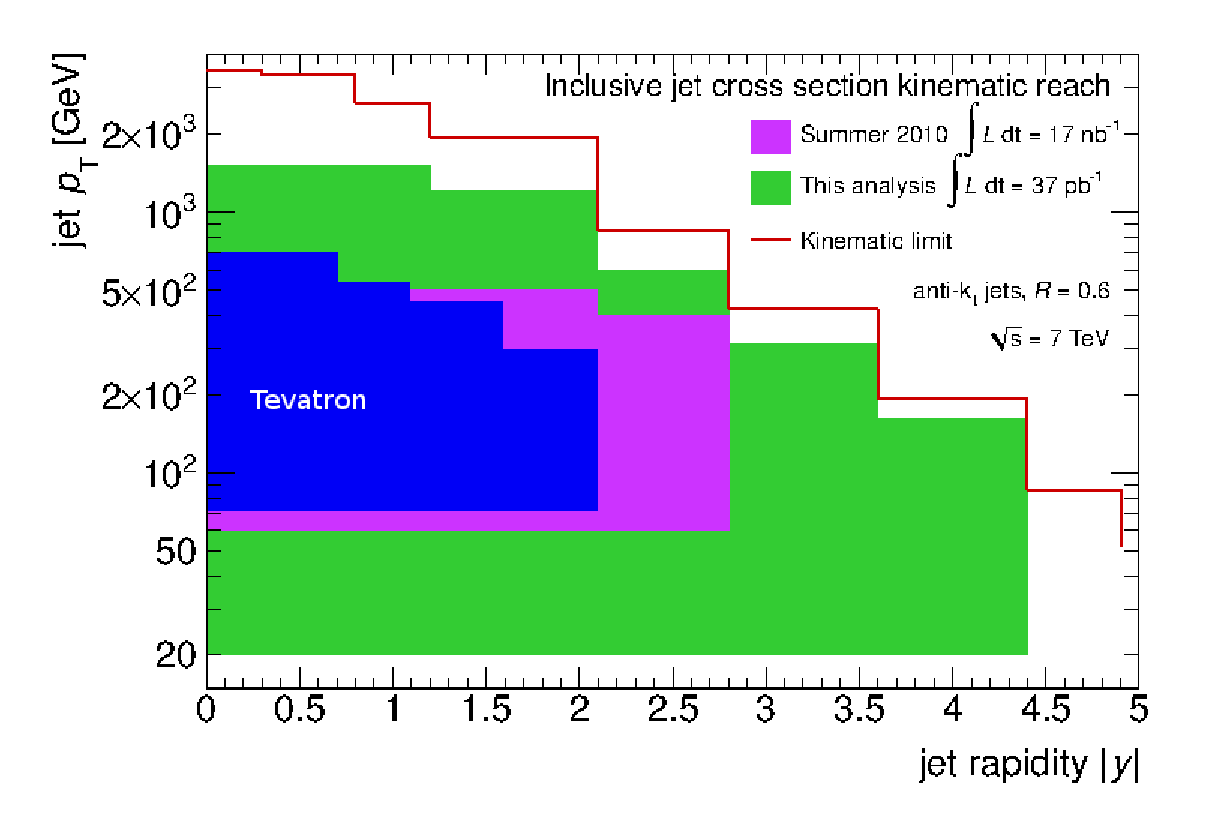
\includegraphics[width=1.0\linewidth,angle=0]{KinematicRangeTevatron.eps}
\column{0.4\linewidth}
\begin{equation*}
y = \frac{1}{2} \log \left(\frac{E + p_z}{E - p_z}\right)
\end{equation*}
\end{columns}
\begin{itemize}
\item Inclusive Jet Cross-Section -  all jets in each event contribute.
\item QCD measurement in a region of phase space not previously explored. Allows study of pQCD + models for soft QCD.
\item First \atlas measurement (purple) used $17 \mathrm{nb}^{-1}$ of early data.
\item This analysis used full 2010 dataset (green) - $37 \mathrm{pb}^{-1}$ of data. Covers kinematic region $\pt > 20 \mathrm{GeV}$ and  $|y| < 4.4$.
\end{itemize}
%\column{0.3\linewidth}
%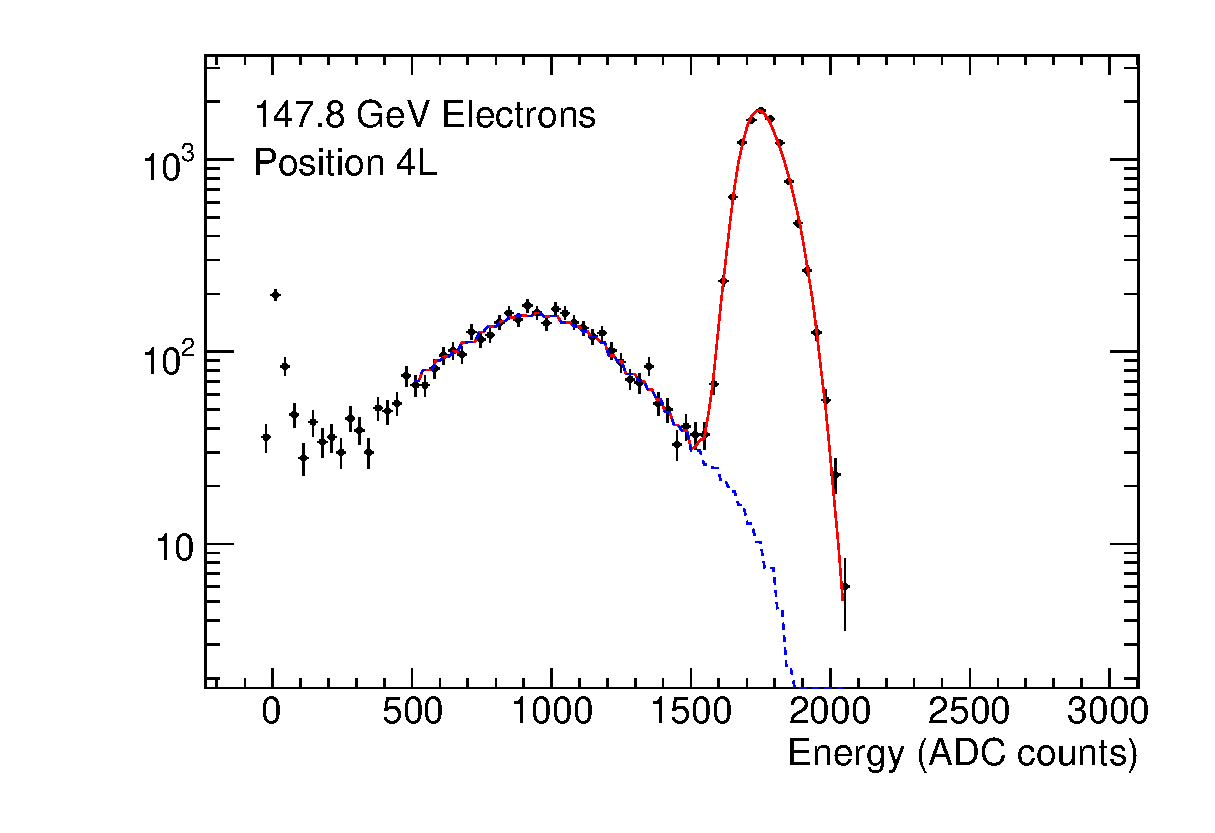
\includegraphics[width=0.8\linewidth,angle=0]{FCalTB_plots/Response_individual_data/Electron_response_148GeV_4L_data.eps}
%\end{columns}
\end{frame}
%%%%%%%%%%%%%%%%%%%%%%%%%%%%%%%%%%%%%%%%%%%%%%%%%%%%%%%%%%%%%%%%%%%
%%%%%%%%%%%%%%%%%%%%%%%%%%%%%%%%%%%%%%%%%%%%%%%%%%%%%%%%%%%%%%%%%%%%
%%\section{Inclusive Jet and Dijet Cross-Section}
%\begin{frame}\frametitle{Inclusive Jet and Dijet Cross-Section}
%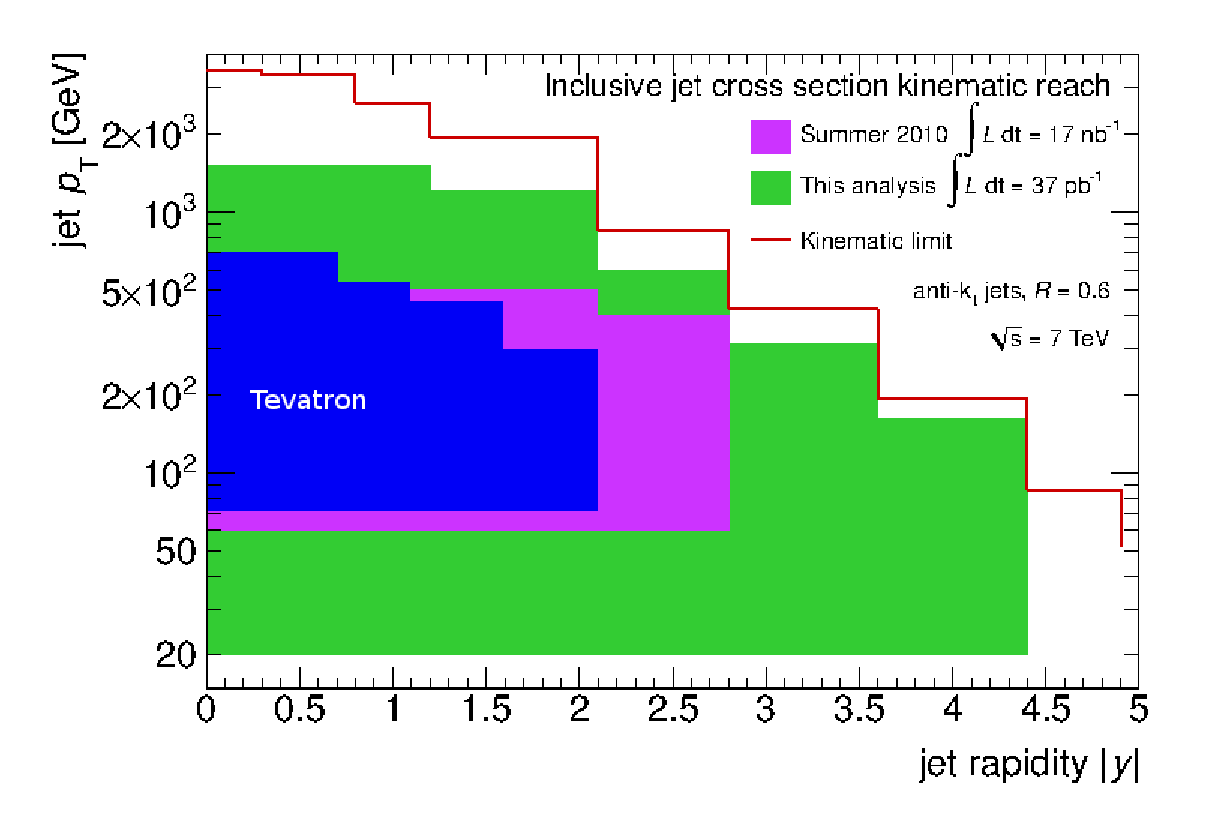
\includegraphics[width=0.6\linewidth,angle=0]{KinematicRangeTevatron.eps}
%\begin{itemize}
%\item Tevatron measured jets with $62 \mathrm{GeV} < \pt <700 \mathrm{GeV}$ and $|y| < 2.1$.
%\item CMS used two seperate analyses in ranges $|y| < 3.0$ and $ 3.2 < \eta < 4.7$ (different jet definitions, gap in coverage).
%\end{itemize}
%%\column{0.3\linewidth}
%%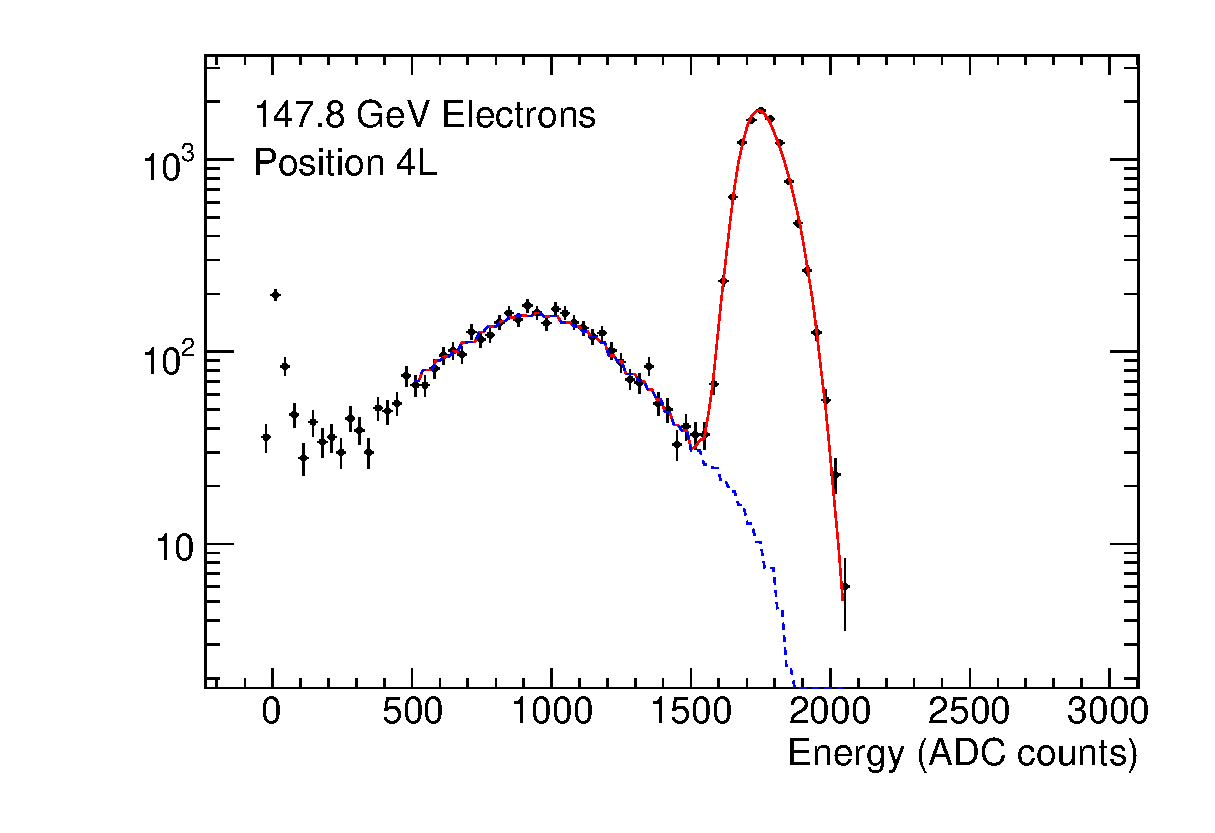
\includegraphics[width=0.8\linewidth,angle=0]{FCalTB_plots/Response_individual_data/Electron_response_148GeV_4L_data.eps}
%%\end{columns}
%\end{frame}
%%%%%%%%%%%%%%%%%%%%%%%%%%%%%%%%%%%%%%%%%%%%%%%%%%%%%%%%%%%%%%%%%%%
%%%%%%%%%%%%%%%%%%%%%%%%%%%%%%%%%%%%%%%%%%%%%%%%%%%%%%%%%%%%%%%%%%%
%\section{Inclusive Jet and Dijet Cross-Section}
%\begin{frame}\frametitle{Dijet Kinematics}
%
%\begin{itemize}
%\item Inclusive cross-section binned in \pt, $y$.
%\item Dijet cross-section binned in $m_\mathrm{12}$, $y^*$.
%\begin{itemize}
%\item describe the dijet kinematics in the COM frame.
%\end{itemize}
%\end{itemize}
%\begin{columns}
%\column{0.3\linewidth}
%\begin{eqnarray*}
%y^* &=& \frac{|y_1 - y_2|}{2}\\
%m_\mathrm{12}^2 &=& \left(p_1 + p_2\right)^2
%\end{eqnarray*}
%\column{0.7\linewidth}
%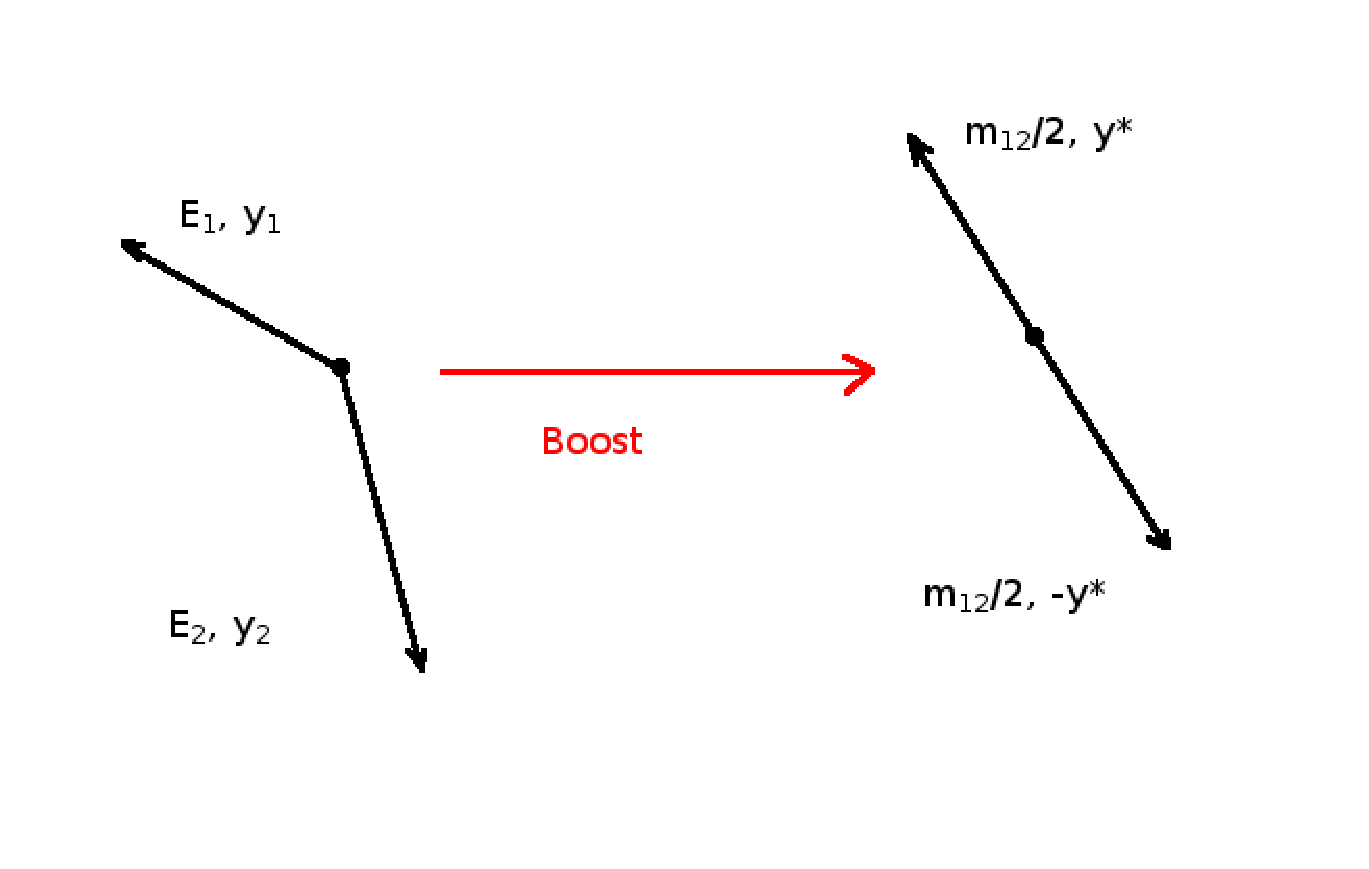
\includegraphics[width=1.0\linewidth,angle=0]{dijet1.eps}
%%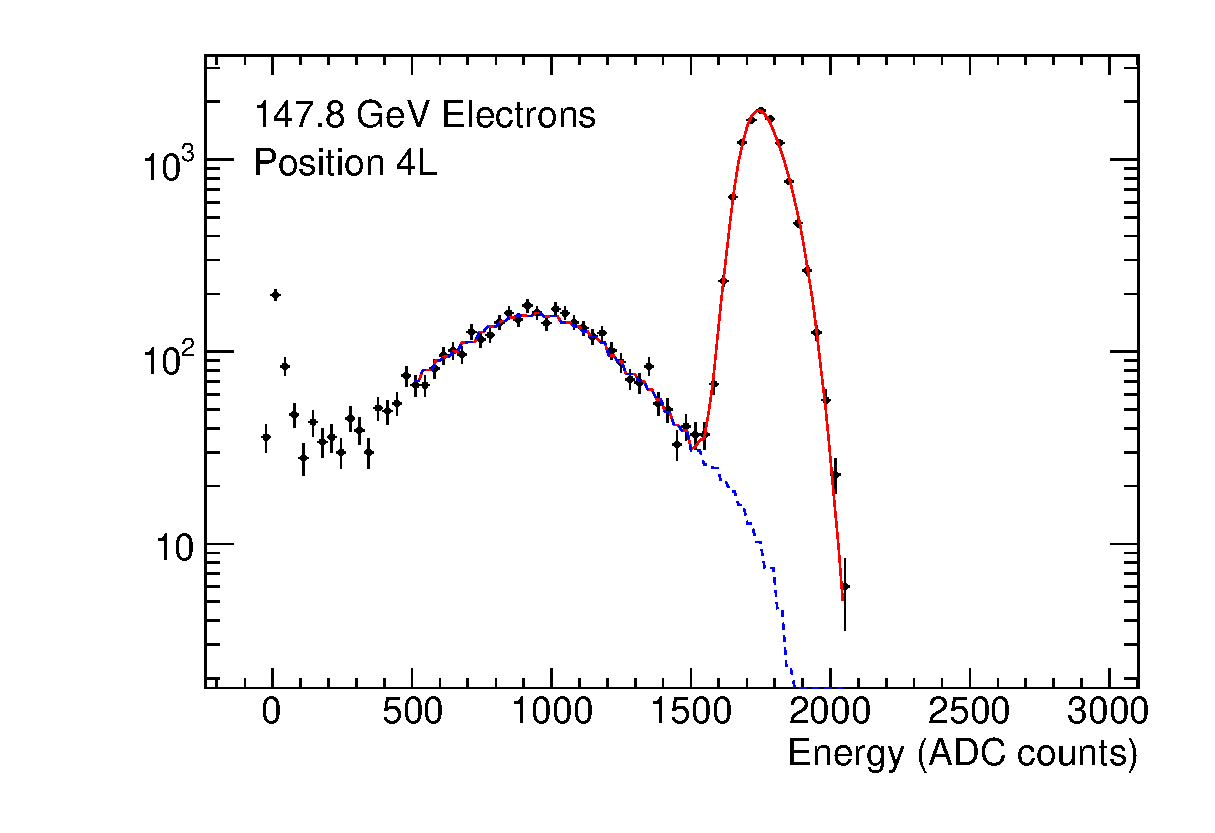
\includegraphics[width=0.8\linewidth,angle=0]{FCalTB_plots/Response_individual_data/Electron_response_148GeV_4L_data.eps}
%\end{columns}
%\end{frame}
%%%%%%%%%%%%%%%%%%%%%%%%%%%%%%%%%%%%%%%%%%%%%%%%%%%%%%%%%%%%%%%%%%%
%\begin{frame}\frametitle{Inclusive Jet and Dijet Cross-Section}
%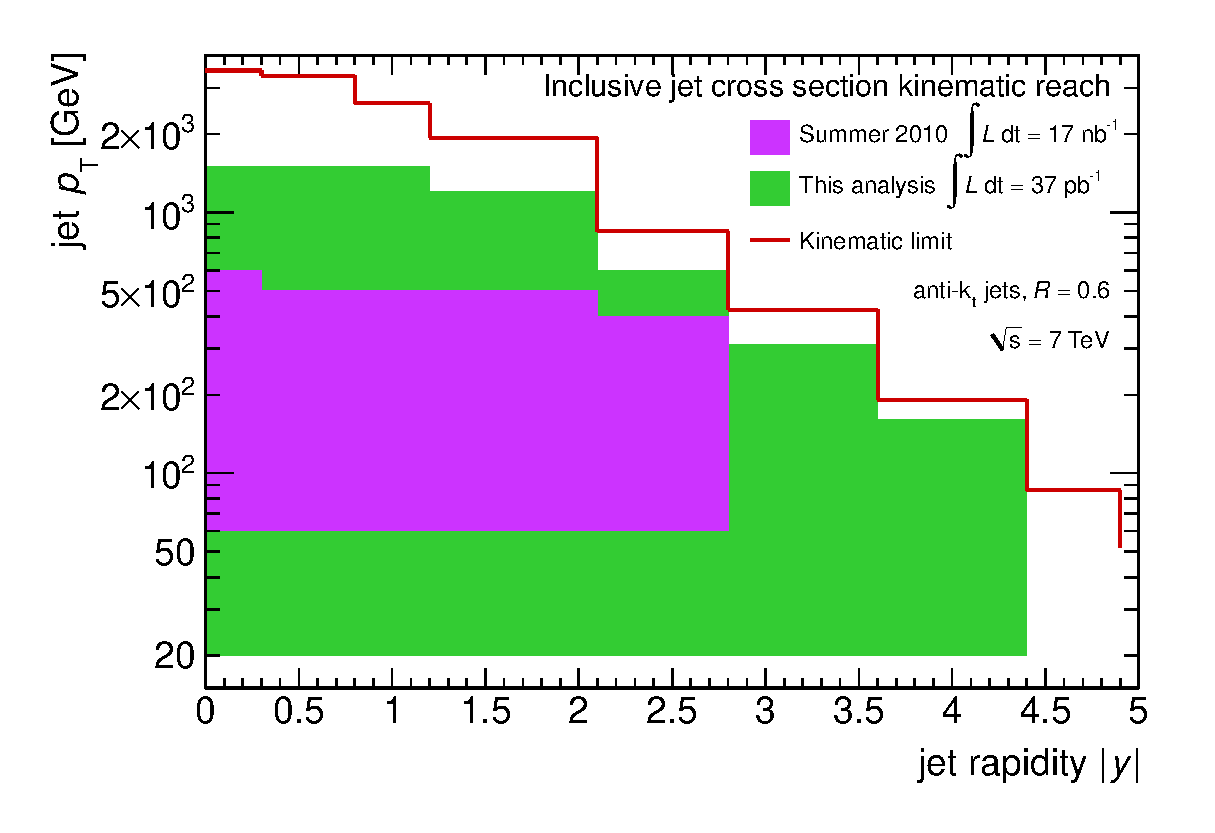
\includegraphics[width=0.6\linewidth,angle=0]{KinematicRange.eps}
%\begin{itemize}
%%\item Inclusive Jet Cross-Section - consider all jets in each event contribute.
%%\item First measurement (purple) used $17 \mathrm{nb}^{-1}$ of early data.
%%\item Full 2010 dataset (green) uses $37 \mathrm{pb}^{-1}$ of data, extends kinematic coverage down to 20 GeV in \pt and to rapidities of $|y| < 4.4$.
%\item Tevatron measured jets with $62 \mathrm{GeV} < \pt <700 \mathrm{GeV}$ and $|y| < 2.1$
%\item CMS measured used two seperate analyses (different jet definitions) in ranges $|y| < 3.0$ and $ 3.2 < \eta < 4.7$
%\end{itemize}
%%\column{0.3\linewidth}
%%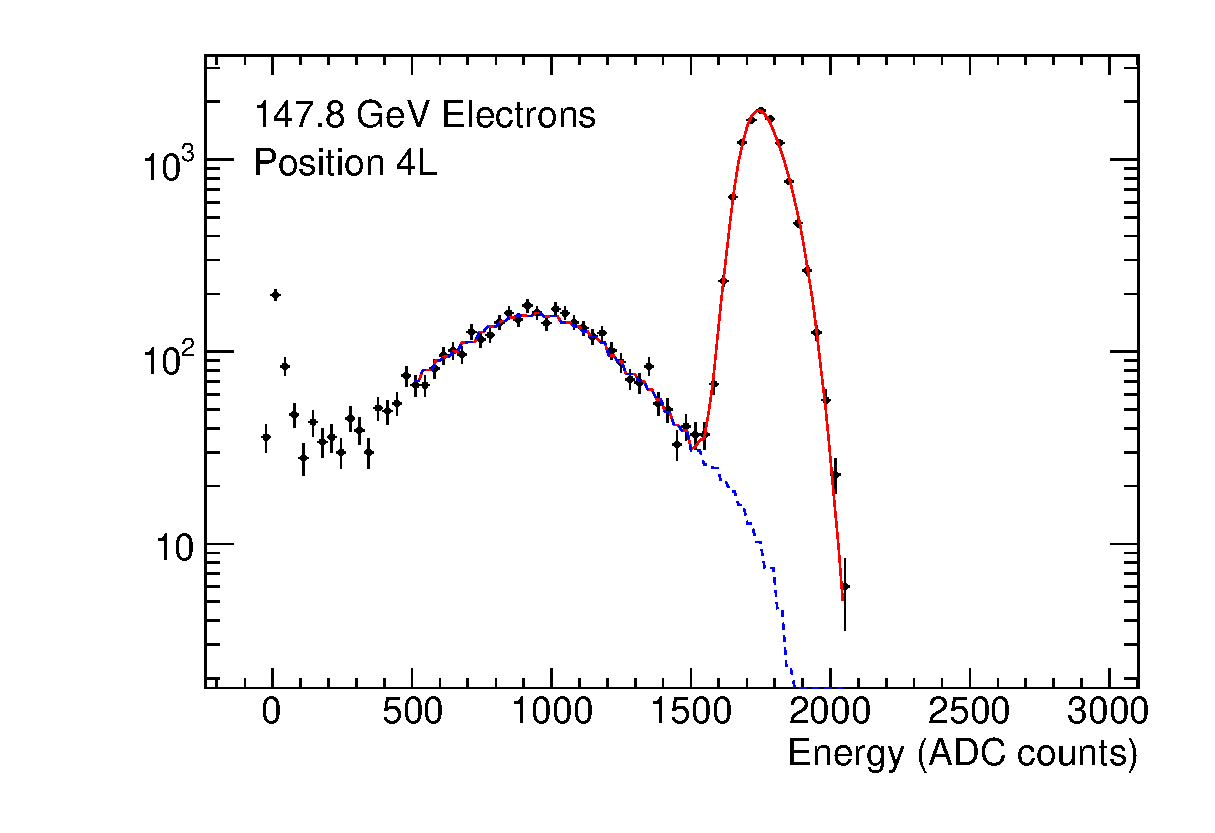
\includegraphics[width=0.8\linewidth,angle=0]{FCalTB_plots/Response_individual_data/Electron_response_148GeV_4L_data.eps}
%%\end{columns}
%\end{frame}
%%%%%%%%%%%%%%%%%%%%%%%%%%%%%%%%%%%%%%%%%%%%%%%%%%%%%%%%%%%%%%%%%%%
\begin{frame}\frametitle{Jet Reconstruction and Calibration}


\begin{itemize}
\item Jets defined using \akt algorithm on topoclusters, with $R = 0.4$ and $R = 0.6$.
\item EM+JES used to calibrate jets - correction factor applied to EM scale jet energy. Binned in $|\eta|$ and \pt.
\item Calibration derived from MC - important to understand simulation.
\item Uncertainty in calibration is generally around 3-5\% at high \pt - Dominant contribution to cross-section uncertainty.
\end{itemize}
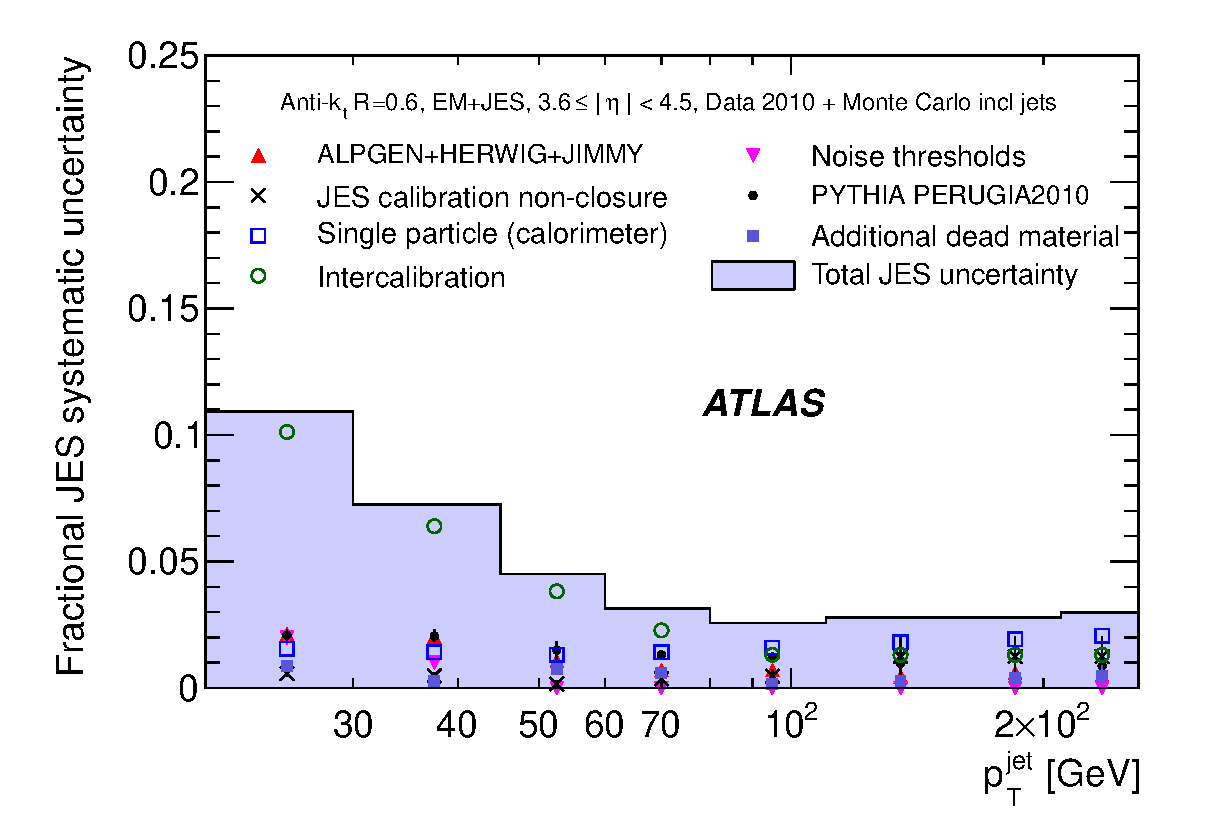
\includegraphics[width=0.6\linewidth,angle=0]{JES_new/fig_22c.eps}

\end{frame}
%%%%%%%%%%%%%%%%%%%%%%%%%%%%%%%%%%%%%%%%%%%%%%%%%%%%%%%%%%%%%%%%%%%
%%%%%%%%%%%%%%%%%%%%%%%%%%%%%%%%%%%%%%%%%%%%%%%%%%%%%%%%%%%%%%%%%%%%
%\subsection{Jet Triggers}
%\begin{frame}\frametitle{Jet Triggers}
%\begin{itemize}
%\item Jet triggers are used to select events containing jets. 
%\item Forward jet triggers (FJ) identify jets in the FCal, central jet triggers (J) identify jets elsewhere.
%\item Level 1 trigger used initially, Level 2 commisioned later
%%\item \alert{ADD SOMETHING HERE}
%%\item \alert{ general comment on JES uncertainty}
%\end{itemize}
%\end{frame}
%%%%%%%%%%%%%%%%%%%%%%%%%%%%%%%%%%%%%%%%%%%%%%%%%%%%%%%%%%%%%%%%%%%%
%%%%%%%%%%%%%%%%%%%%%%%%%%%%%%%%%%%%%%%%%%%%%%%%%%%%%%%%%%%%%%%%%%%
\begin{frame}\frametitle{Jet Triggers}
\begin{itemize}
\item Forward jet triggers (FJ) identify jets in the FCal, central jet triggers (J) identify jets elsewhere.
\item Trigger towers are formed from analog sums of calorimeter channels
\item ``Jet Elements'' are formed by grouping trigger towers (0.2$\times$0.2 in $\eta-\phi$)
\item Sliding window algorithm used to find jets at L1, identify a Region of Interest (ROI)
\item At L2, cone based algorithm run on cells within the ROI
\end{itemize}
\begin{center}
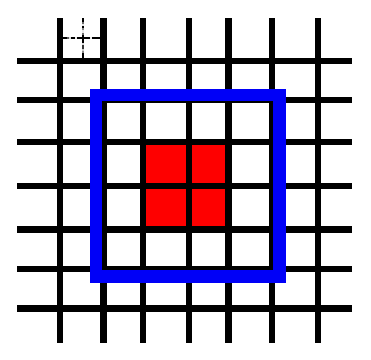
\includegraphics[width=0.35\linewidth,angle=0]{sliding_window.eps}
%\item Level 1 trigger used initially, Level 2 commisioned later
%\item \alert{ general comment on JES uncertainty}
\end{center}
\end{frame}
%%%%%%%%%%%%%%%%%%%%%%%%%%%%%%%%%%%%%%%%%%%%%%%%%%%%%%%%%%%%%%%%%%%
%%%%%%%%%%%%%%%%%%%%%%%%%%%%%%%%%%%%%%%%%%%%%%%%%%%%%%%%%%%%%%%%%%%
\begin{frame}\frametitle{Trigger Efficiency}
\begin{itemize}
\item The inclusive efficiency of a trigger is defined as 
\begin{equation*}
\epsilon_\mathrm{inc} = \frac{N_\mathrm{triggered,inc}}{N_\mathrm{reference}},
\end{equation*}
\item $N_\mathrm{reference}$ is the number of jets in a reference sample.
\item $N_\mathrm{triggered,inc}$ is the number of jets from events in reference sample that meet the trigger condition. \item Binning $N_\mathrm{triggered,inc}$ and $N_\mathrm{reference}$ in \pt~ allows the efficiency to be described as a function of \pt.

\item Triggers are used to select events above their ``plateau point''. Sum bins of $N_\mathrm{triggered,inc}$ and $N_\mathrm{reference}$ and take the ratio. The plateau point is where this ratio drops below 99\%, such that trigger is at least 99\% efficient above this point.
\end{itemize}
\end{frame}
%%%%%%%%%%%%%%%%%%%%%%%%%%%%%%%%%%%%%%%%%%%%%%%%%%%%%%%%%%%%%%%%%%%

%%%%%%%%%%%%%%%%%%%%%%%%%%%%%%%%%%%%%%%%%%%%%%%%%%%%%%%%%%%%%%%%%%%
\begin{frame}\frametitle{Trigger Efficiency - Forward Bin ($3.6 < |y|< 4.4$)}
\begin{columns}
\column{0.5\linewidth}
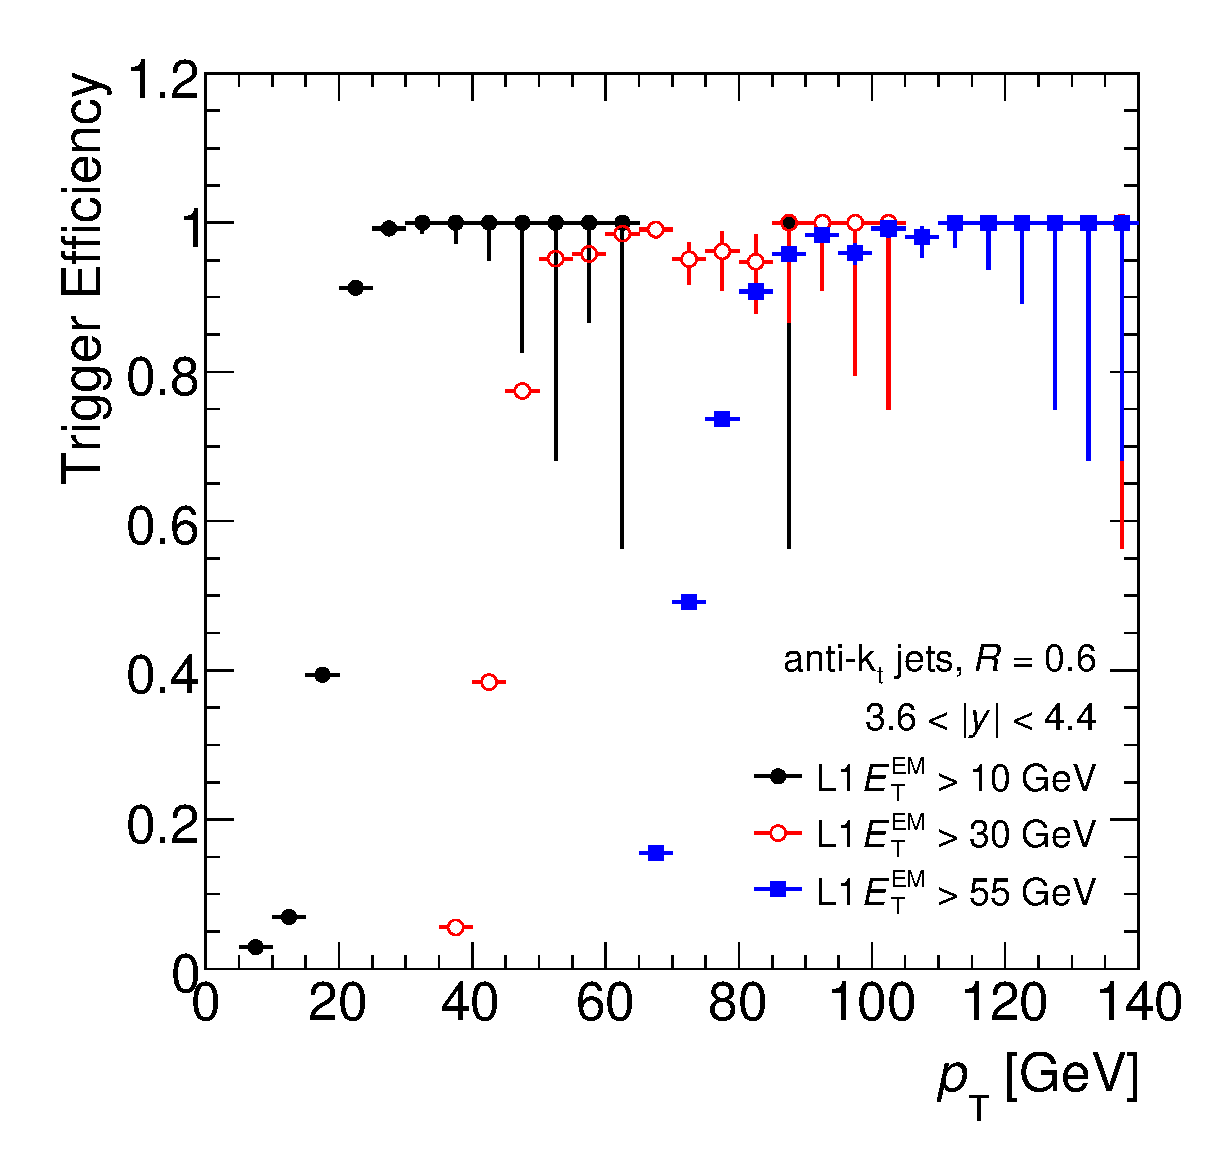
\includegraphics[width=0.8\linewidth,angle=0]{L1_triggers_forward_bin_akt6.eps}
\column{0.5\linewidth}
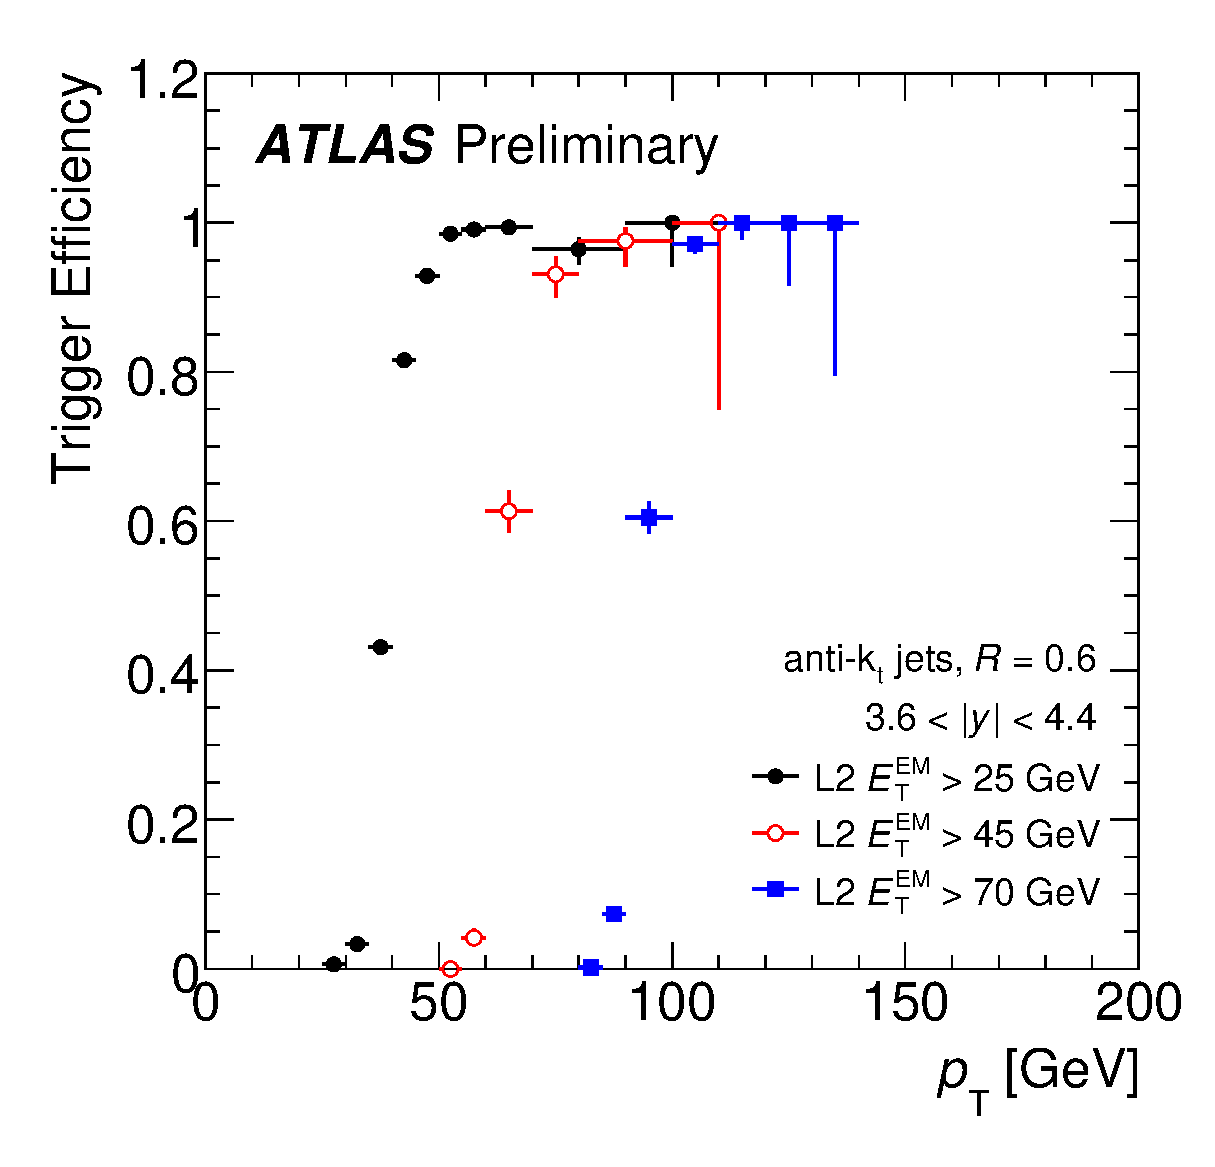
\includegraphics[width=0.8\linewidth,angle=0]{L1L2_triggers_forward_binm_akt6.eps}
\end{columns}
\begin{itemize}
\item Trigger efficiencies at L1 (left) and L2 (right), for jets with $R=0.6$ in the FCal ($3.6 < |y| < 4.4$)
\item L1 triggers reach plateau at 23 GeV, 60 GeV and 99 GeV, and are used to collect data above 30 GeV, 80 GeV and 110 GeV, respectively.
%\item L2 trigger reach plateau at 45 GeV,77 GeV and 103 GeV, and are used above 60 GeV, 110 GeV and 160 GeV, respectively.
\end{itemize}
\end{frame}
%%%%%%%%%%%%%%%%%%%%%%%%%%%%%%%%%%%%%%%%%%%%%%%%%%%%%%%%%%%%%%%%%%%

%%%%%%%%%%%%%%%%%%%%%%%%%%%%%%%%%%%%%%%%%%%%%%%%%%%%%%%%%%%%%%%%%%%
\begin{frame}\frametitle{Transition Bin Triggers}
\begin{center}
\begin{columns}
\column{0.5\linewidth}
\begin{center}
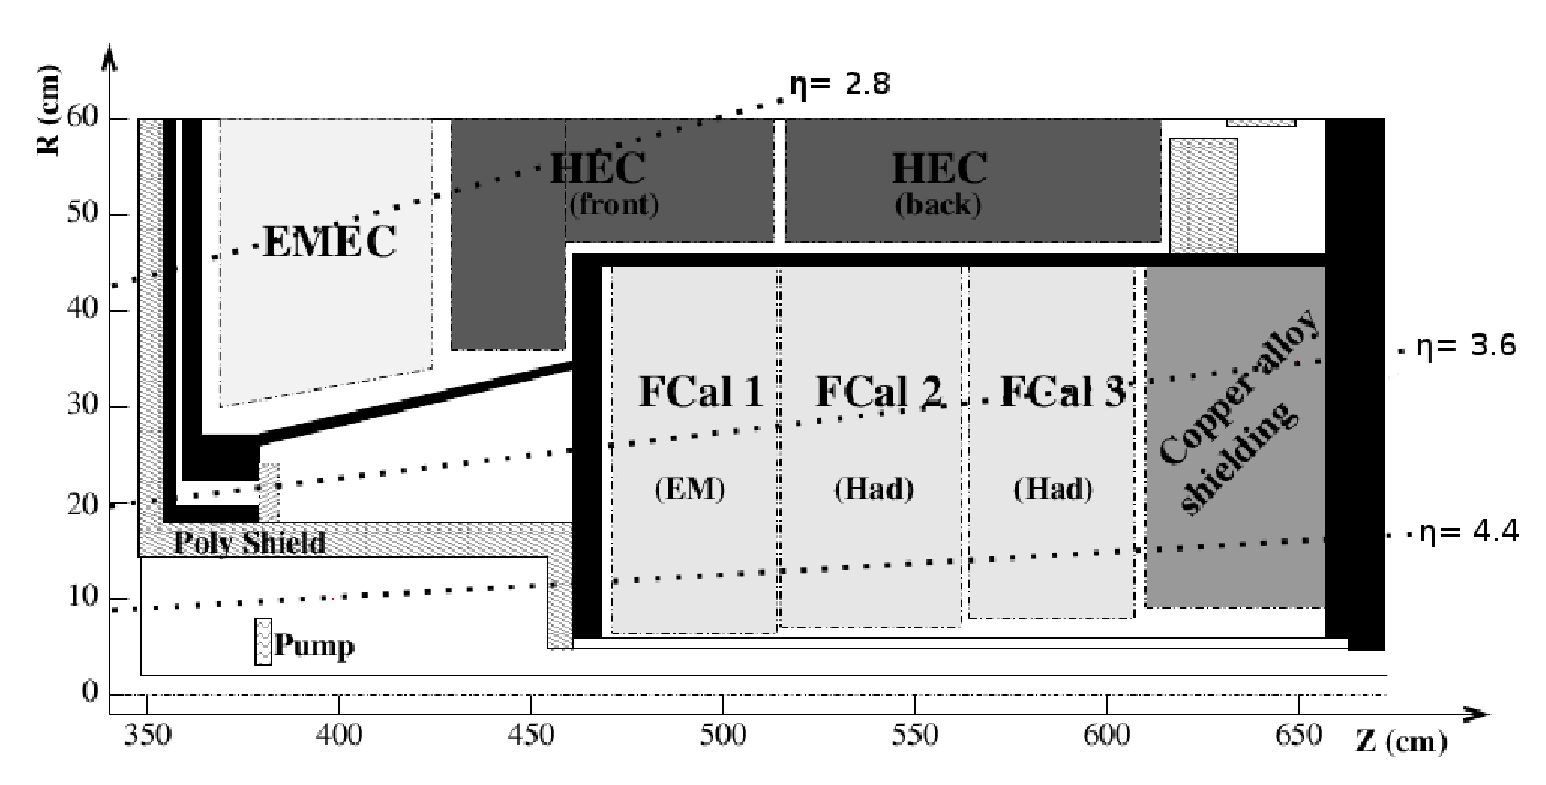
\includegraphics[width=0.95\linewidth,angle=0]{atlas_EC_xsec2.eps}
\end{center}
\column{0.5\linewidth}
\begin{center}
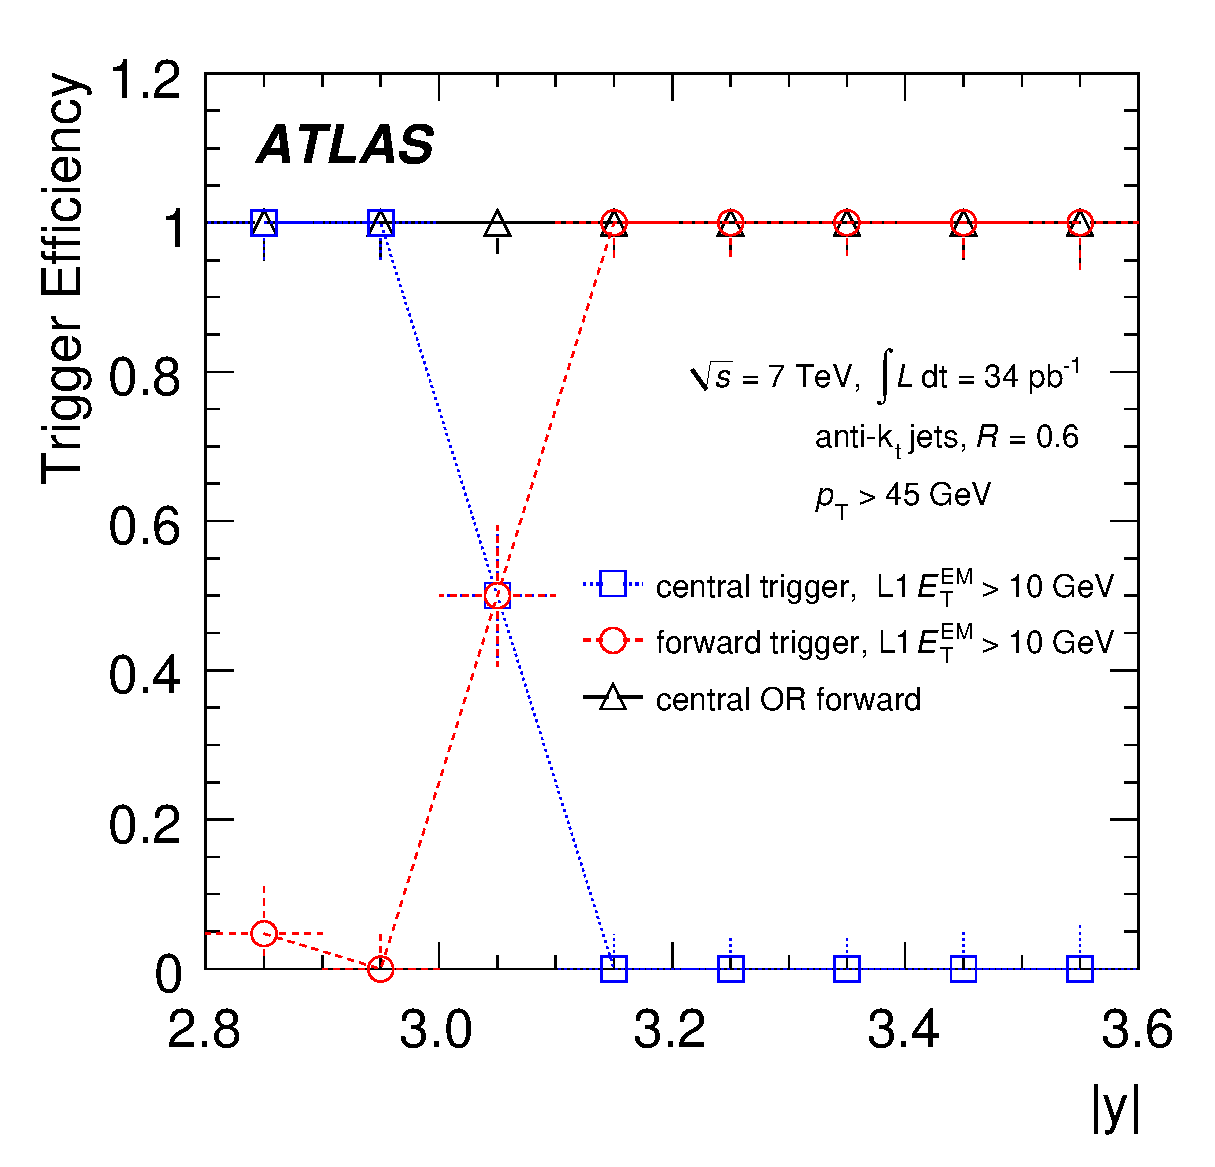
\includegraphics[width=0.7\linewidth,angle=0]{eta_efficiency_akt6.eps}
\end{center}
\end{columns}
\end{center}
\begin{itemize}
\item Transition bin covers the region $2.8 < |y| <3.6$.
%\item CMS analyses don't cover all of this region.
\item Neither the Central jet trigger or the Forward Jet trigger are fully efficient in this range.
\item Need to use a combination of the two (``OR'') to select jets in this region.
\end{itemize}
\end{frame}
%%%%%%%%%%%%%%%%%%%%%%%%%%%%%%%%%%%%%%%%%%%%%%%%%%%%%%%%%%%%%%%%%%%
\begin{frame}\frametitle{Trigger Efficiency - Transition Bin ($2.8 < |y| < 3.6$)}
\begin{columns}
\column{0.5\linewidth}
\includegraphics[width=0.7\linewidth,angle=0]{L1_triggers_transition_bin_akt6.eps}
\column{0.5\linewidth}
\includegraphics[width=0.7\linewidth,angle=0]{L1L2_triggers_transition_binm_akt6.eps}
\end{columns}
\begin{itemize}
\item Trigger efficiencies at L1 (left) and L2 (right), for jets with $R=0.6$ in the Transition bin ($2.8 < |y| < 3.6$)
%\item L1 triggers reach plateau at 23 GeV, 60 GeV and 99 GeV, and are used to collect data above 30 GeV, 80 GeV and 110 GeV, respectively.
%\item L2 trigger reach plateau at 45 GeV, 77 GeV and 103 GeV, and are used above 60 GeV, 110 GeV and 160 GeV, respectively.
\end{itemize}
\end{frame}
%%%%%%%%%%%%%%%%%%%%%%%%%%%%%%%%%%%%%%%%%%%%%%%%%%%%%%%%%%%%%%%%%%%
\begin{frame}\frametitle{Transition Bin Cross-Section}
\begin{itemize}
\item When a single trigger is used, Jet cross-section is given by
\begin{equation*}
\sigma = N_{jets}\left(\sum_i\frac{\intL_i}{S_i}\right)^{-1},
\end{equation*}
where the sum runs over LumiBlocks, $\intL_i$ is the integrated luminosity and $S_i$ is the trigger prescale.

\item When using the OR of the triggers, events are divided into three classes: those which meet the forward trigger condition (10), the central trigger condition (01), and both trigger conditions (11). The jet cross-section is then
\begin{equation}
\sigma =  \frac{N_\mathrm{01}}{\intL_\mathrm{01}} + \frac{N_\mathrm{10}}{\intL_\mathrm{10}} +\frac{N_\mathrm{11}}{\intL_\mathrm{11}}
\end{equation}
where $N_{xx}$ is the number of jets counted from events of that type, and
%\begin{eqnarray*}
%\intL_\mathrm{01} &=& \sum_i\frac{\intL_i}{S_{i\mathrm{,01}}}\\
%\intL_\mathrm{10} &=& \sum_i\frac{\intL_i}{S_{i\mathrm{,10}}}\\
%\intL_\mathrm{11} &=& \sum_i\frac{\intL_i \left(S_{i\mathrm{,01}} + S_{i\mathrm{,10}} - 1\right) }{ S_{i\mathrm{,01}} \, S_{i\mathrm{,10}}}
%\end{eqnarray*}
\begin{equation*}
%\intL_\mathrm{01} =\sum_i\frac{\intL_i}{S_{i\mathrm{,01}}} ,\quad \intL_\mathrm{10} = \sum_i\frac{\intL_i}{S_{i\mathrm{,10}}}, \quad 
\intL_\mathrm{11} = \sum_i\frac{\intL_i \left(S_{i\mathrm{,01}} + S_{i\mathrm{,10}} - 1\right) }{ S_{i\mathrm{,01}} \, S_{i\mathrm{,10}}} .
\end{equation*}
\end{itemize}
\end{frame}
%%%%%%%%%%%%%%%%%%%%%%%%%%%%%%%%%%%%%%%%%%%%%%%%%%%%%%%%%%%%%%%%%%%
%%%%%%%%%%%%%%%%%%%%%%%%%%%%%%%%%%%%%%%%%%%%%%%%%%%%%%%%%%%%%%%%%%%%
%\begin{frame}\frametitle{Unfolding}
%\begin{itemize}
%\item Jet energies are measured with finite resolution. Jet spectrum falls sharply with \pt, so more low \pt~jets are measured to have high \pt~than high \pt~jets are measured to have low \pt. Measured spectrum is skewed towards high \pt.
%\item Unfolding is used to correct this effect, based on Monte Carlo. ``Truth'' jets are fromed from the particles output by the event generator. The interaction of these jets with the detector is then simulated (\geant), and ``reconstructed'' are obtained using the same methods as for data. Detector effects can then be inferred by matching truth jets to reconstructed jets and forming a ``Transfer Matrix''.
%\item Transfer matrix can then be inverted and applied to measured jet spectrum to obtain a corrected spectrum. This is not a trivial task, the Iterative, Dynamically Stabilised (IDS) method is used.
%\end{itemize}
%\end{frame}
%%%%%%%%%%%%%%%%%%%%%%%%%%%%%%%%%%%%%%%%%%%%%%%%%%%%%%%%%%%%%%%%%%%%
%%%%%%%%%%%%%%%%%%%%%%%%%%%%%%%%%%%%%%%%%%%%%%%%%%%%%%%%%%%%%%%%%%%
\subsection{Cross-Section Results}
\begin{frame}\frametitle{Inclusive Jet Cross-Section Results}
\begin{columns}
\column{0.5\linewidth}
\includegraphics[width=0.95\linewidth,angle=0]{inclusive_results/figs_new/fig_10_inc_cross_section_akt6.eps}
\column{0.5\linewidth}
\includegraphics[width=0.95\linewidth,angle=0]{inclusive_results/figs_new/fig_12d_inc_ratio_akt6_forward.eps}%fig_15.eps}
\end{columns}
\begin{itemize}
\item Theoretical predictions obtained using NLOJet++ with CT10 Parton Distribution Functions, generally good agreement.
\item Of the results obtained from NLOJet++, the MSTW2008 pdf gives the best agreement with data.
\item Best agreement between data and theory obtained from Powheg, when interfaced to Pythia (AUET2B tune).
\end{itemize}
\end{frame}
%%%%%%%%%%%%%%%%%%%%%%%%%%%%%%%%%%%%%%%%%%%%%%%%%%%%%%%%%%%%%%%%%%%
%%%%%%%%%%%%%%%%%%%%%%%%%%%%%%%%%%%%%%%%%%%%%%%%%%%%%%%%%%%%%%%%%%%%
%\subsection{Dijet Cross-Section Results}
%
%\begin{frame}\frametitle{Dijet Cross-Section Results}
%\begin{center}
%\includegraphics[width=0.4\linewidth,angle=0]{inclusive_results/figs_new/fig_15.eps}
%\end{center}
%\begin{itemize}
%\item Theoretical predictions obtained using NLOJet++ with CT10 PDF set, generally good agreement.
%\item Best agreement between data and NLOJet++ obtained using MSTW2008 PDF set.
%\item Best agreement between data and Powheg results obtained with powheg is interfaced to Pythia (AUET2B tune).
%\end{itemize}
%\end{frame}
%%%%%%%%%%%%%%%%%%%%%%%%%%%%%%%%%%%%%%%%%%%%%%%%%%%%%%%%%%%%%%%%%%%%
%%%%%%%%%%%%%%%%%%%%%%%%%%%%%%%%%%%%%%%%%%%%%%%%%%%%%%%%%%%%%%%%%%%
%\section{Summary}
\begin{frame}\frametitle{Summary}
\begin{itemize}
\item Data from 2003 beam test of ATLAS forward calorimeter has been analysed, and compared to results obtained from Monte Carlo. The simulation agrees well with the data, and effects associated with additional upstream material are well modelled, providing validation of the simulation.  %\alert{focus on this when discussing TB results earlier}
\item Inclusive Jet and Dijet (backup) cross-sections have been measured using 37 $\mathrm{pb}^{-1}$ of data collected in 2010. These measurements cover a large kinematic region, coherently probing rapidity region that has not previously been studied at a hadron-hadron collider. Cross-section measurements at CMS use two seperate analyses (different jet definitions) to study jets in the central and forward regions, and there is a gap in the rapidity coverage spanned by these analyses.
\end{itemize}
\end{frame}
%%%%%%%%%%%%%%%%%%%%%%%%%%%%%%%%%%%%%%%%%%%%%%%%%%%%%%%%%%%%%%%%%%%
%%%%%%%%%%%%%%%%%%%%%%%%%%%%%%%%%%%%%%%%%%%%%%%%%%%%%%%%%%%%%%%%%%%
%%%%%%%%%%%%%%%%%%%%%%%%%%%%%%%%%%%%%%%%%%%%%%%%%%%%%%%%%%%%%%%%%%%%
%%%%%%%%%%%%%%%%%%%%%%%%%%%%%%%%%%%%%%%%%%%%%%%%%%%%%%%%%%%%%%%%%%%%
%%%%%%%%%%%%%%%%%%%%%%%%%%%%%%%%%%%%%%%%%%%%%%%%%%%%%%%%%%%%%%%%%%%
%%%%%%%%%%%%%%%%%%%%%%%%%%%%%%%%%%%%%%%%%%%%%%%%%%%%%%%%%%%%%%%%%%%
%%%%%%%%%%%%%%%%%%%%%%%%%%%%%%%%%%%%%%%%%%%%%%%%%%%%%%%%%%%%%%%%%%%%
\begin{frame}
\frametitle{Backup slides}
Backup Slides
\end{frame}
%%%%%%%%%%%%%%%%%%%%%%%%%%%%%%%%%%%%%%%%%%%%%%%%%%%%%%%%%%%%%%%%%%%
%%%%%%%%%%%%%%%%%%%%%%%%%%%%%%%%%%%%%%%%%%%%%%%%%%%%%%%%%%%%%%%%%%%%
%\begin{frame}\frametitle{Things that should go in the backup slides}
%\begin{itemize}
%\item dijet - add a slide on y* and mass - diagrams showing dijet kinematics in COM frame. This could be not a backup.
%\item data/theory comparisons of Inclusive jet and dijet - ratio plots
%\item something on pp collisions (pileup/UE), event generators
%\end{itemize}
%\end{frame}
%%\end{fmffile}
%
%%%%%%%%%%%%%%%%%%%%%%%%%%%%%%%%%%%%%%%%%%%%%%%%%%%%%%%%%%%%%%%%%%%%
\begin{frame} 
\frametitle{Proton-Proton Collisions}
In addition to hard scattering between partons, other processes involved.
\begin{itemize}
%\item In addition to hard scattering between partons, other processes involved.
\item Partons collinearly radiate before (after) hard scatter - initial (final) state radiation.
\item Soft scatterings can occur between partons not involved in the hard scatter (Multiple parton interactions - Underlying Event)
\item Pile-up
\begin{itemize}
\item At design specifications, \atlas expects $\sim$ 23 proton-proton collisions per bunch crossing (only $\sim 3-4$ during 2010).
\item An event containing a hard scattering will also contain several soft scatterings between other protons.
\item This additional pile-up energy is corrected for in the EM+JES calibration.
\end{itemize}
\end{itemize}
 

\end{frame}
%%%%%%%%%%%%%%%%%%%%%%%%%%%%%%%%%%%%%%%%%%%%%%%%%%%%%%%%%%%%%%%%%%%
%\subsection{ FCal electrodes  }
\begin{frame} 
\frametitle{FCal structure} 
\begin{columns}
\column{0.6\linewidth}
\includegraphics[width=0.8\linewidth,angle=0]{fcalfrontclose2.eps}\\
\begin{itemize}
\item Electrodes run down length of modules.
\item Thin gaps between rod and tube occupied by LAr, sensitive regions.
\item Absorbing material is copper in FCal1, tungsten based in FCal2 \& FCal3
\end{itemize}
\column{0.4\linewidth}
\includegraphics[width=0.5\linewidth,angle=0]{FCal1_face.eps}\\
\includegraphics[width=0.5\linewidth,angle=0]{FCal_electrode.eps}\\
\includegraphics[width=0.5\linewidth,angle=0]{/TBoverview/rods_slugs.eps}\\
%\includegraphics[width=0.5\linewidth,angle=0]{FCal_face.eps}\\
\end{columns}
\end{frame}
%%%%%%%%%%%%%%%%%%%%%%%%%%%%%%%%%%%%%%%%%%%%%%%%%%%%%%%%%%%%%%%%%%%%
%%%%%%%%%%%%%%%%%%%%%%%%%%%%%%%%%%%%%%%%%%%%%%%%%%%%%%%%%%%%%%%%%%
\begin{frame} 
\frametitle{Topological clustering}
\begin{itemize}
\item Cells clustered based on energy/noise significance.
\item ``420'' scheme used for hadronic clusters
\begin{itemize}
\item If a cell has $|E|/\sigma > 4.0$, it is considered a seed.
\item Adjacent cells are added to the cluster if $|E|/\sigma > 2.0$ (neighbours).
\item Neighbour step is repeated until there are no cells adjacent to the cluster with $|E|/\sigma > 2.0$
\item all ``perimeter'' cells are added to the cluster (require $|E|/\sigma > 0.0$).
\end{itemize}
\item Topoclusters are used at \atlas
\item Don't require tracking information for formation.
\end{itemize}
 

\end{frame}
%%%%%%%%%%%%%%%%%%%%%%%%%%%%%%%%%%%%%%%%%%%%%%%%%%%%%%%%%%%%%%%%%%%%


\begin{frame}\frametitle{Unfolding}
\begin{itemize}
\item Jet energies are measured with finite resolution. Jet spectrum falls sharply with \pt, so more low \pt~jets are measured to have high \pt~than high \pt~jets are measured to have low \pt. Measured spectrum is skewed towards high \pt.
\item Unfolding is used to correct this effect, based on Monte Carlo. ``Truth'' jets are fromed from the particles output by the event generator. The interaction of these jets with the detector is then simulated (\geant), and ``reconstructed'' are obtained using the same methods as for data. Detector effects can then be inferred by matching truth jets to reconstructed jets and forming a ``Transfer Matrix''.
\item Transfer matrix can then be inverted and applied to measured jet spectrum to obtain a corrected spectrum. This is not a trivial task, the Iterative, Dynamically Stabilised (IDS) method is used.
\end{itemize}
\end{frame}
%%%%%%%%%%%%%%%%%%%%%%%%%%%%%%%%%%%%%%%%%%%%%%%%%%%%%%%%%%%%%%%%%%%
%%%%%%%%%%%%%%%%%%%%%%%%%%%%%%%%%%%%%%%%%%%%%%%%%%%%%%%%%%%%%%%%%%
\begin{frame} 
\frametitle{Inclusive Jet results - NLOJet++}
\begin{columns}
\column{0.5\linewidth}
\includegraphics[width=1.0\linewidth,angle=0]{inclusive_results/figs_new/fig_12c_inc_ratio_akt6_central.eps}
\column{0.5\linewidth}
\includegraphics[width=1.0\linewidth,angle=0]{inclusive_results/figs_new/fig_12d_inc_ratio_akt6_forward.eps}
\end{columns}
Ratio of data to NLOJet++ using CT10 pdf. Ratios of NLOJet++ with other pdfs to CT10 are also shown.
\end{frame}
%%%%%%%%%%%%%%%%%%%%%%%%%%%%%%%%%%%%%%%%%%%%%%%%%%%%%%%%%%%%%%%%%%%
%%%%%%%%%%%%%%%%%%%%%%%%%%%%%%%%%%%%%%%%%%%%%%%%%%%%%%%%%%%%%%%%%%
\begin{frame} 
\frametitle{Inclusive Jet results - Powheg}
\begin{columns}
\column{0.5\linewidth}
\includegraphics[width=1.0\linewidth,angle=0]{inclusive_results/figs_new/fig_13c_ratio_powheg_akt6a.eps}
\column{0.5\linewidth}
\includegraphics[width=1.0\linewidth,angle=0]{inclusive_results/figs_new/fig_13d_ratio_powheg_akt6b.eps}
\end{columns}
Theoretical predictions obtained using \powheg, interfaced to parton shower MC generators.
%\begin{centering}
%\subfigure{
%\includegraphics[width=0.45\linewidth,angle=0]{inclusive_results/figs_new/fig_13c_ratio_powheg_akt6a.eps}
%\label{fig_xsec_rat_akt6_pc}
%}
%\subfigure{
%\includegraphics[width=0.45\linewidth,angle=0]{inclusive_results/figs_new/fig_13d_ratio_powheg_akt6b.eps}
%\label{fig_xsec_rat_akt6_pf}

\end{frame}
%%%%%%%%%%%%%%%%%%%%%%%%%%%%%%%%%%%%%%%%%%%%%%%%%%%%%%%%%%%%%%%%%%%%
\begin{frame}\frametitle{Electron Response Linearity}
%\subsection{Results}
\begin{columns}
\column{0.5\linewidth}
\includegraphics[width=0.95\linewidth,angle=0]{FCalTB_plots/electron_linearity_4L.eps}
\column{0.5\linewidth}
\includegraphics[width=0.95\linewidth,angle=0]{FCalTB_plots/electron_linearity_residuals_4L.eps}
\end{columns}

\begin{itemize}
\item Response vs beam energy - expect a linear relationship. 
\item Slope at 4L gives the EM calibration currently used at \atlas.
\item Good agreement between Data and MC.
\item Changes from 4L$\rightarrow$4H (not shown) similar in Data and MC.
\end{itemize}
%\begin{columns}
%\column{0.4\linewidth}
%\begin{itemize}
%%\item Response linearity vs beam energy
%\item Slope at position 4L consistent with prediction.
%\item Change in intercept from 4L$\rightarrow$4H similiar in Data and MC
%\end{itemize}
%\column{0.6\linewidth}
%\begin{tabular}{|l|l|l|l|}
%\hline
%linearity result & slope (ADC/GeV)& Intercept (ADC) \\
%\hline
%Data (4L) & 11.966 $\pm$ 0.002 & -9.26 $\pm$ 0.07 \\
%Simulation (4L) & 11.865 $\pm$ 0.003 & -6.45 $\pm$ 0.13 \\
%Data (4H) & 11.693 $\pm$ 0.002 & -17.53 $\pm$ 0.10 \\
%Simulation (4H) & 11.747 $\pm$ 0.003 & -15.44 $\pm$ 0.13 \\
%\hline
%\end{tabular}
%\end{columns}

%\item Cylindrical clusters formed by summing energies of cells within radius of 8 cm (electrons) and 16 cm (hadrons).
%\item Response is fit with a Double Gaussian (impact point dependence of response). For electron beams, hadron contamination is modelled in the fit. 
%\end{itemize}
%\column{0.3\linewidth}
%\includegraphics[width=0.8\linewidth,angle=0]{FCalTB_plots/Response_individual_data/Electron_response_148GeV_4L_data.eps}
%\end{columns}
\end{frame}
%
%%%%%%%%%%%%%%%%%%%%%%%%%%%%%%%%%%%%%%%%%%%%%%%%%%%%%%%%%%%%%%%%%%%%
%%%%%%%%%%%%%%%%%%%%%%%%%%%%%%%%%%%%%%%%%%%%%%%%%%%%%%%%%%%%%%%%%%%

\begin{frame}\frametitle{Electron Response Linearity (4H)}
%\subsection{Results}
\begin{columns}
\column{0.5\linewidth}
\includegraphics[width=0.95\linewidth,angle=0]{FCalTB_plots/electron_linearity_4H.eps}
\column{0.5\linewidth}
\includegraphics[width=0.95\linewidth,angle=0]{FCalTB_plots/electron_linearity_residuals_4H.eps}
\end{columns}

\begin{itemize}


\item Good agreement between Data and MC.
\item Changes from 4L$\rightarrow$4H similar in Data and MC.
\end{itemize}
\end{frame}
%%%%%%%%%%%%%%%%%%%%%%%%%%%%%%%%%%%%%%%%%%%%%%%%%%%%%%%%%%%%%%%%%%%%
\begin{frame}\frametitle{Electron results}
{\footnotesize
\begin{tabular}{|l|l|l|l|}
\hline
linearity result & slope (ADC/GeV)& Intercept (ADC) \\
\hline
Data (4L) & 11.966 $\pm$ 0.002 & -9.26 $\pm$ 0.07 \\
Simulation (4L) & 11.865 $\pm$ 0.003 & -6.45 $\pm$ 0.13 \\
Data (4H) & 11.693 $\pm$ 0.002 & -17.53 $\pm$ 0.10 \\
Simulation (4H) & 11.747 $\pm$ 0.003 & -15.44 $\pm$ 0.13 \\
\hline
\end{tabular}
\begin{tabular}{|l|l|l|l|}
\hline
& Stochastic Term (\% $\mathrm{GeV}^{1/2}$) & Constant Term (\%) \\
\hline
Data (4L) & 27.0 $\pm$ 0.2 & 3.58 $\pm$ 0.02\\
Simulation (4L) & 24.7 $\pm$ 0.3 & 4.56 $\pm$ 0.03\\
Data (4H) & 33.7 $\pm$ 0.2 & 3.11 $\pm$ 0.03\\
Simulation (4H) & 28.1 $\pm$ 0.3 & 3.96 $\pm$ 0.03\\
\hline
\end{tabular}
}
Linearity and resolution results for electrons
\end{frame}
%%%%%%%%%%%%%%%%%%%%%%%%%%%%%%%%%%%%%%%%%%%%%%%%%%%%%%%%%%%%%%%%%%%%

\begin{frame}\frametitle{Hadron Resolution results}
Results from hadron resolution fits, for data and MC at 4L and 4H.
{\footnotesize
\begin{tabular}{|l|l|l|l|}
\hline
& Stochastic Term (\% $\mathrm{GeV}^{1/2}$) & Constant Term (\%) \\
\hline
Data (4L) & 88.0 $\pm$ 0.6 & 6.79 $\pm$ 0.06\\
QGSP\_BERT (4L) & 86.2 $\pm$ 1.1 & 6.54 $\pm$ 0.18\\
QGSP\_BERT\_HP (4L) & 90.5 $\pm$ 1.1 & 6.22 $\pm$ 0.13\\
FTFP\_BERT (4L) & 81.2 $\pm$ 1.1 & 6.04 $\pm$ 0.11\\
%Data (4H) & 121.3 $\pm$ 0.6 & 7.13 $\pm$ 0.07\\
%QGSP\_BERT (4H) & 127.2 $\pm$ 1.1 & 6.41 $\pm$ 0.17\\
%QGSP\_BERT\_HP (4H) & 119.6 $\pm$ 1.2 & 7.71 $\pm$ 0.15\\
%FTFP\_BERT (4H) & 115.8 $\pm$ 1.1 & 7.12 $\pm$ 0.14\\
Data (4H) & 120.7 $\pm$ 0.6 & 6.98 $\pm$ 0.07\\
QGSP\_BERT (4H) & 127.6 $\pm$ 1.1 & 6.62 $\pm$ 0.17\\
QGSP\_BERT\_HP (4H) & 123.3 $\pm$ 1.2 & 7.58 $\pm$ 0.16\\
FTFP\_BERT (4H) & 119.2 $\pm$ 1.1 & 6.77 $\pm$ 0.15\\
\hline
\end{tabular}
}
\end{frame}
%%%%%%%%%%%%%%%%%%%%%%%%%%%%%%%%%%%%%%%%%%%%%%%%%%%%%%%%%%%%%%%%%%%%
%%%%%%%%%%%%%%%%%%%%%%%%%%%%%%%%%%%%%%%%%%%%%%%%%%%%%%%%%%%%%%%%%%
%\section{Inclusive Jet and Dijet Cross-Section}
\begin{frame}\frametitle{Dijet Kinematics}

\begin{itemize}
\item Inclusive cross-section binned in \pt, $y$.
\item Dijet cross-section binned in $m_\mathrm{12}$, $y^*$.
\begin{itemize}
\item describe the dijet kinematics in the COM frame.
\end{itemize}
\end{itemize}
\begin{columns}
\column{0.3\linewidth}
\begin{eqnarray*}
y^* &=& \frac{|y_1 - y_2|}{2}\\
m_\mathrm{12}^2 &=& \left(p_1 + p_2\right)^2
\end{eqnarray*}
\column{0.7\linewidth}
\includegraphics[width=1.0\linewidth,angle=0]{dijet1.eps}
%\includegraphics[width=0.8\linewidth,angle=0]{FCalTB_plots/Response_individual_data/Electron_response_148GeV_4L_data.eps}
\end{columns}
\end{frame}
%%%%%%%%%%%%%%%%%%%%%%%%%%%%%%%%%%%%%%%%%%%%%%%%%%%%%%%%%%%%%%%%%%%
%%%%%%%%%%%%%%%%%%%%%%%%%%%%%%%%%%%%%%%%%%%%%%%%%%%%%%%%%%%%%%%%%%%
%\subsection{Dijet Cross-Section Results}
\begin{frame}\frametitle{Dijet Cross-Section Results}
\begin{columns}
\column{0.5\linewidth}
\includegraphics[width=0.95\linewidth,angle=0]{inclusive_results/figs_new/fig_15.eps}
\column{0.5\linewidth}
\includegraphics[width=0.95\linewidth,angle=0]{inclusive_results/figs_new/fig_17b.eps}%fig_15.eps}
\end{columns}
\begin{itemize}
\item Trigger scheme used for dijet analysis is similar to that used in the transition bin of the inclusive analysis - Dijet event is considered if either leading jet or subleading jet meets relevant trigger condition.
\item Theoretical predictions obtained using NLOJet++ with CT10 Parton Distribution Functions, generally good agreement.
\item Best agreement between data and theory obtained from Powheg, when interfaced to Pythia (AUET2B tune).
\end{itemize}
\end{frame}
%%%%%%%%%%%%%%%%%%%%%%%%%%%%%%%%%%%%%%%%%%%%%%%%%%%%%%%%%%%%%%%%%%%

%%%%%%%%%%%%%%%%%%%%%%%%%%%%%%%%%%%%%%%%%%%%%%%%%%%%%%%%%%%%%%%%%%%%
%\begin{frame}\frametitle{Cluster Moments}
%\begin{columns}
%\column{0.5\linewidth}
%\includegraphics[width=0.8\linewidth,angle=0]{FCalTB_plots/hadron_resolution_4L.eps}
%\column{0.5\linewidth}
%\includegraphics[width=0.8\linewidth,angle=0]{FCalTB_plots/hadron_resolution_4H.eps}
%\end{columns}
%\begin{itemize}
%\item Hadronic calibration - flat weights.
%\item Weights from MC generally agree with those from data.
%\item Weights derived from data at 200 GeV are used to reconstruct (most) data and MC results.
%\end{itemize}
%%\column{0.3\linewidth}
%%\includegraphics[width=0.8\linewidth,angle=0]{FCalTB_plots/Response_individual_data/Electron_response_148GeV_4L_data.eps}
%%\end{columns}
%\end{frame}
%%%%%%%%%%%%%%%%%%%%%%%%%%%%%%%%%%%%%%%%%%%%%%%%%%%%%%%%%%%%%%%%%%%

\end{document}









